

\documentclass[twoside,twocolumn,9pt]{article}
\usepackage{extsizes}
\usepackage[super,sort&compress,comma]{natbib} 
\usepackage[version=3]{mhchem}
\usepackage[left=1.5cm, right=1.5cm, top=1.785cm, bottom=2.0cm]{geometry}
\usepackage{balance}
\usepackage{widetext}
\usepackage{times,mathptmx}
\usepackage{sectsty}
\usepackage{graphicx} 
\usepackage{lastpage}
\usepackage[format=plain,justification=raggedright,singlelinecheck=false,font={stretch=1.125,small,sf},labelfont=bf,labelsep=space]{caption}
\usepackage{float}
\usepackage{fancyhdr}
\usepackage{fnpos}
\usepackage[english]{babel}
\usepackage{array}
\usepackage{droidsans}
\usepackage{charter}
\usepackage[T1]{fontenc}
\usepackage[usenames,dvipsnames]{xcolor}
\usepackage{setspace}
\usepackage[compact]{titlesec}
\usepackage{gensymb}
%DIF 30a30
\usepackage{amsmath,amssymb} %DIF > 
%DIF -------
%\usepackage[hidelinks]{hyperref}
%DIF 31a32-38
 %DIF > 
%%%%%%%%%%%%%%%%%%%%%%%%%%% %DIF > 
% remove this in the final version %DIF > 
%\usepackage{lineno} %DIF > 
%\linenumbers %DIF > 
%%%%%%%%%%%%%%%%%%%%%%%%%%% %DIF > 
 %DIF > 
%DIF -------

%%%Please don't disable any packages in the preamble, as this may cause the template to display incorrectly.%%%


\usepackage{epstopdf}%This line makes .eps figures into .pdf - please comment out if not required.

\pdfminorversion=5 
\pdfobjcompresslevel=3  
\pdfcompresslevel=9


\definecolor{cream}{RGB}{222,217,201}
%DIF PREAMBLE EXTENSION ADDED BY LATEXDIFF
%DIF UNDERLINE PREAMBLE %DIF PREAMBLE
\RequirePackage[normalem]{ulem} %DIF PREAMBLE
\RequirePackage{color}\definecolor{RED}{rgb}{1,0,0}\definecolor{BLUE}{rgb}{0,0,1} %DIF PREAMBLE
\providecommand{\DIFadd}[1]{{\protect\color{blue}\uwave{#1}}} %DIF PREAMBLE
\providecommand{\DIFdel}[1]{{\protect\color{red}\sout{#1}}}                      %DIF PREAMBLE
%DIF SAFE PREAMBLE %DIF PREAMBLE
\providecommand{\DIFaddbegin}{} %DIF PREAMBLE
\providecommand{\DIFaddend}{} %DIF PREAMBLE
\providecommand{\DIFdelbegin}{} %DIF PREAMBLE
\providecommand{\DIFdelend}{} %DIF PREAMBLE
%DIF FLOATSAFE PREAMBLE %DIF PREAMBLE
\providecommand{\DIFaddFL}[1]{\DIFadd{#1}} %DIF PREAMBLE
\providecommand{\DIFdelFL}[1]{\DIFdel{#1}} %DIF PREAMBLE
\providecommand{\DIFaddbeginFL}{} %DIF PREAMBLE
\providecommand{\DIFaddendFL}{} %DIF PREAMBLE
\providecommand{\DIFdelbeginFL}{} %DIF PREAMBLE
\providecommand{\DIFdelendFL}{} %DIF PREAMBLE
\newcommand{\DIFscaledelfig}{0.5}
%DIF HIGHLIGHTGRAPHICS PREAMBLE %DIF PREAMBLE
\RequirePackage{settobox} %DIF PREAMBLE
\RequirePackage{letltxmacro} %DIF PREAMBLE
\newsavebox{\DIFdelgraphicsbox} %DIF PREAMBLE
\newlength{\DIFdelgraphicswidth} %DIF PREAMBLE
\newlength{\DIFdelgraphicsheight} %DIF PREAMBLE
% store original definition of \includegraphics %DIF PREAMBLE
\LetLtxMacro{\DIFOincludegraphics}{\includegraphics} %DIF PREAMBLE
\newcommand{\DIFaddincludegraphics}[2][]{{\color{blue}\fbox{\DIFOincludegraphics[#1]{#2}}}} %DIF PREAMBLE
\newcommand{\DIFdelincludegraphics}[2][]{% %DIF PREAMBLE
\sbox{\DIFdelgraphicsbox}{\DIFOincludegraphics[#1]{#2}}% %DIF PREAMBLE
\settoboxwidth{\DIFdelgraphicswidth}{\DIFdelgraphicsbox} %DIF PREAMBLE
\settoboxtotalheight{\DIFdelgraphicsheight}{\DIFdelgraphicsbox} %DIF PREAMBLE
\scalebox{\DIFscaledelfig}{% %DIF PREAMBLE
\parbox[b]{\DIFdelgraphicswidth}{\usebox{\DIFdelgraphicsbox}\\[-\baselineskip] \rule{\DIFdelgraphicswidth}{0em}}\llap{\resizebox{\DIFdelgraphicswidth}{\DIFdelgraphicsheight}{% %DIF PREAMBLE
\setlength{\unitlength}{\DIFdelgraphicswidth}% %DIF PREAMBLE
\begin{picture}(1,1)% %DIF PREAMBLE
\thicklines\linethickness{2pt} %DIF PREAMBLE
{\color[rgb]{1,0,0}\put(0,0){\framebox(1,1){}}}% %DIF PREAMBLE
{\color[rgb]{1,0,0}\put(0,0){\line( 1,1){1}}}% %DIF PREAMBLE
{\color[rgb]{1,0,0}\put(0,1){\line(1,-1){1}}}% %DIF PREAMBLE
\end{picture}% %DIF PREAMBLE
}\hspace*{3pt}}} %DIF PREAMBLE
} %DIF PREAMBLE
\LetLtxMacro{\DIFOaddbegin}{\DIFaddbegin} %DIF PREAMBLE
\LetLtxMacro{\DIFOaddend}{\DIFaddend} %DIF PREAMBLE
\LetLtxMacro{\DIFOdelbegin}{\DIFdelbegin} %DIF PREAMBLE
\LetLtxMacro{\DIFOdelend}{\DIFdelend} %DIF PREAMBLE
\DeclareRobustCommand{\DIFaddbegin}{\DIFOaddbegin \let\includegraphics\DIFaddincludegraphics} %DIF PREAMBLE
\DeclareRobustCommand{\DIFaddend}{\DIFOaddend \let\includegraphics\DIFOincludegraphics} %DIF PREAMBLE
\DeclareRobustCommand{\DIFdelbegin}{\DIFOdelbegin \let\includegraphics\DIFdelincludegraphics} %DIF PREAMBLE
\DeclareRobustCommand{\DIFdelend}{\DIFOaddend \let\includegraphics\DIFOincludegraphics} %DIF PREAMBLE
\LetLtxMacro{\DIFOaddbeginFL}{\DIFaddbeginFL} %DIF PREAMBLE
\LetLtxMacro{\DIFOaddendFL}{\DIFaddendFL} %DIF PREAMBLE
\LetLtxMacro{\DIFOdelbeginFL}{\DIFdelbeginFL} %DIF PREAMBLE
\LetLtxMacro{\DIFOdelendFL}{\DIFdelendFL} %DIF PREAMBLE
\DeclareRobustCommand{\DIFaddbeginFL}{\DIFOaddbeginFL \let\includegraphics\DIFaddincludegraphics} %DIF PREAMBLE
\DeclareRobustCommand{\DIFaddendFL}{\DIFOaddendFL \let\includegraphics\DIFOincludegraphics} %DIF PREAMBLE
\DeclareRobustCommand{\DIFdelbeginFL}{\DIFOdelbeginFL \let\includegraphics\DIFdelincludegraphics} %DIF PREAMBLE
\DeclareRobustCommand{\DIFdelendFL}{\DIFOaddendFL \let\includegraphics\DIFOincludegraphics} %DIF PREAMBLE
%DIF END PREAMBLE EXTENSION ADDED BY LATEXDIFF

\begin{document}

\pagestyle{fancy}
\thispagestyle{plain}
\fancypagestyle{plain}{

%%%HEADER%%%
\fancyhead[C]{
\includegraphics[width=18.5cm]{head_foot/header_bar}}
\fancyhead[L]{\hspace{0cm}\vspace{1.5cm}
\includegraphics[height=30pt]{head_foot/journal_name}}
\fancyhead[R]{\hspace{0cm}\vspace{1.7cm}
\includegraphics[height=55pt]{head_foot/RSC_LOGO_CMYK}}
\renewcommand{\headrulewidth}{0pt}
}
%%%END OF HEADER%%%

%%%PAGE SETUP - Please do not change any commands within this section%%%
\makeFNbottom
\makeatletter
\renewcommand\LARGE{\@setfontsize\LARGE{15pt}{17}}
\renewcommand\Large{\@setfontsize\Large{12pt}{14}}
\renewcommand\large{\@setfontsize\large{10pt}{12}}
\renewcommand\footnotesize{\@setfontsize\footnotesize{7pt}{10}}
\makeatother

\renewcommand{\thefootnote}{\fnsymbol{footnote}}
\renewcommand\footnoterule{\vspace*{1pt}% 
\color{cream}\hrule width 3.5in height 0.4pt \color{black}\vspace*{5pt}} 
\setcounter{secnumdepth}{5}

\makeatletter 
\renewcommand\@biblabel[1]{#1}            
\renewcommand\@makefntext[1]% 
{\noindent\makebox[0pt][r]{\@thefnmark\,}#1}
\makeatother 
\renewcommand{\figurename}{\small{Fig.}~}
\sectionfont{\sffamily\Large}
\subsectionfont{\normalsize}
\subsubsectionfont{\bf}
\setstretch{1.125} %In particular, please do not alter this line.
\setlength{\skip\footins}{0.8cm}
\setlength{\footnotesep}{0.25cm}
\setlength{\jot}{10pt}
\titlespacing*{\section}{0pt}{4pt}{4pt}
\titlespacing*{\subsection}{0pt}{15pt}{1pt}
%%%END OF PAGE SETUP%%%

%%%FOOTER%%%
\fancyfoot{}
\fancyfoot[LO,RE]{\vspace{-7.1pt}
\includegraphics[height=9pt]{head_foot/LF}}
\fancyfoot[CO]{\vspace{-7.1pt}\hspace{13.2cm}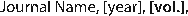
\includegraphics{head_foot/RF}}
\fancyfoot[CE]{\vspace{-7.2pt}\hspace{-14.2cm}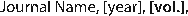
\includegraphics{head_foot/RF}}
\fancyfoot[RO]{\footnotesize{\sffamily{1--\pageref{LastPage} ~\textbar  \hspace{2pt}\thepage}}}
\fancyfoot[LE]{\footnotesize{\sffamily{\thepage~\textbar\hspace{3.45cm} 1--\pageref{LastPage}}}}
\fancyhead{}
\renewcommand{\headrulewidth}{0pt} 
\renewcommand{\footrulewidth}{0pt}
\setlength{\arrayrulewidth}{1pt}
\setlength{\columnsep}{6.5mm}
\setlength\bibsep{1pt}
%%%END OF FOOTER%%%

%%%FIGURE SETUP - please do not change any commands within this section%%%
\makeatletter 
\newlength{\figrulesep} 
\setlength{\figrulesep}{0.5\textfloatsep} 

\newcommand{\topfigrule}{\vspace*{-1pt}% 
\noindent{\color{cream}\rule[-\figrulesep]{\columnwidth}{1.5pt}} }

\newcommand{\botfigrule}{\vspace*{-2pt}% 
\noindent{\color{cream}\rule[\figrulesep]{\columnwidth}{1.5pt}} }

\newcommand{\dblfigrule}{\vspace*{-1pt}% 
\noindent{\color{cream}\rule[-\figrulesep]{\textwidth}{1.5pt}} }

\makeatother
%%%END OF FIGURE SETUP%%%

%%%TITLE, AUTHORS AND ABSTRACT%%%
\DIFdelbegin %DIFDELCMD < \twocolumn[
%DIFDELCMD <   \begin{@twocolumnfalse}
%DIFDELCMD < \vspace{3cm}
%DIFDELCMD < \sffamily
%DIFDELCMD < \begin{tabular}{m{4.5cm} p{13.5cm} }
%DIFDELCMD < 

%DIFDELCMD < 
\includegraphics{head_foot/DOI} & \noindent\LARGE{\textbf{Friction controls submerged granular flows$^\dag$}} \\%Article title goes here instead of the text "This is the title"
%DIFDELCMD < \vspace{0.3cm} & \vspace{0.3cm} \\
%DIFDELCMD < 

%DIFDELCMD <  & \noindent\large{
%DIFDELCMD < Juha Koivisto,$^{\ast}$\textit{$^{a,b}$}
%DIFDELCMD < Marko Korhonen,\textit{$^{a}$}
%DIFDELCMD < Mikko Alava,\textit{$^{a}$}
%DIFDELCMD < Carlos P. Ortiz,\textit{$^{b}$}
%DIFDELCMD < Douglas J. Durian\textit{$^{b}$}
%DIFDELCMD < and Antti Puisto\textit{$^{a}$}} \\%Author names go here instead of "Full name", etc.
%DIFDELCMD < 

%DIFDELCMD < 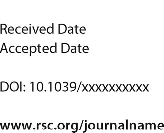
\includegraphics{head_foot/dates} & \noindent\normalsize{We investigate the coupling between interstitial medium and granular 
%DIFDELCMD < particles by studying the hopper flow of dry and submerged system 
%DIFDELCMD < experimentally and numerically.
%DIFDELCMD < In accordance with earlier studies, we find, that the dry hopper 
%DIFDELCMD < empties at a constant rate. However, in the submerged system we 
%DIFDELCMD < observe the surging of the flow rate. 
%DIFDELCMD < We model both systems using the discrete element method, which we couple 
%DIFDELCMD < with computational fluid dynamics in the case of a submerged hopper. 
%DIFDELCMD < We are able to match the simulations and the experiments with good 
%DIFDELCMD < accuracy. 
%DIFDELCMD < To do that, we fit the particle-particle contact friction for each 
%DIFDELCMD < system separately, finding that submerging the hopper changes the
%DIFDELCMD < particle-particle contact friction from $\mu_{vacuum}=0.15$ to 
%DIFDELCMD < $\mu_{sub}=0.13$, while all the other simulation parameters remain 
%DIFDELCMD < the same. Furthermore, our experiments find a particle size dependence 
%DIFDELCMD < to the flow rate, which is comprehended based on arguments on the terminal 
%DIFDELCMD < velocity and drag. 
%DIFDELCMD < These results jointly allow us to conclude that at 
%DIFDELCMD < the large particle limit, the interstitial medium does not matter, in 
%DIFDELCMD < contrast to small particles. 
%DIFDELCMD < The particle size limit, where this occurs depends on the viscosity 
%DIFDELCMD < of the interstitial fluid.} \\%The abstract goes here instead of the text "The abstract should be..."
%DIFDELCMD < 

%DIFDELCMD < \end{tabular}
%DIFDELCMD < 

%DIFDELCMD <  \end{@twocolumnfalse} \vspace{0.6cm}
%DIFDELCMD < 

%DIFDELCMD <   ]
%DIFDELCMD < %%%
\DIFdelend \DIFaddbegin \twocolumn[
  \begin{@twocolumnfalse}
\vspace{3cm}
\sffamily
\begin{tabular}{m{4.5cm} p{13.5cm} }


\includegraphics{head_foot/DOI} & \noindent\LARGE{\textbf{Friction controls even submerged granular flows$^\dag$}} \\%Article title goes here instead of the text "This is the title"
\vspace{0.3cm} & \vspace{0.3cm} \\

 & \noindent\large{Juha Koivisto,$^{\ast}$\textit{$^{a,b}$}
Marko Korhonen,\textit{$^{a}$}
Mikko Alava,\textit{$^{a}$}
Carlos P. Ortiz,\textit{$^{b}$}
Douglas J. Durian\textit{$^{b}$}
and Antti Puisto\textit{$^{a}$}} \\%Author names go here instead of "Full name", etc.

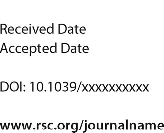
\includegraphics{head_foot/dates} & \noindent\normalsize{We investigate the coupling between interstitial medium and granular 
particles by studying the hopper flow of dry and submerged system 
experimentally and numerically.
In accordance with earlier studies, we find, that the dry hopper 
empties at a constant rate. However, in the submerged system we 
observe the surging of the flow rate. 
We model both systems using the discrete element method, which we couple 
with computational fluid dynamics in the case of a submerged hopper. 
We are able to match the simulations and the experiments with good 
accuracy. 
To do that, we fit the particle-particle contact friction for each 
system separately, finding that submerging the hopper changes the
particle-particle contact friction from $\mu_{vacuum}=0.15$ to 
$\mu_{sub}=0.13$, while all the other simulation parameters remain 
the same. Furthermore, our experiments find a particle size dependence 
to the flow rate. We rationalize this finding based on arguments on the terminal 
velocity and drag: As is well known, larger particles are less prone to
be influenced by the interstitial fluid.
} \\%The abstract goes here instead of the text "The abstract should be..."
\end{tabular}

 \end{@twocolumnfalse} \vspace{0.6cm}

  ]
\DIFaddend %%%END OF TITLE, AUTHORS AND ABSTRACT%%%

%%%FONT SETUP - please do not change any commands within this section
\renewcommand*\rmdefault{bch}\normalfont\upshape
\rmfamily
\section*{}
\vspace{-1cm}


%%%FOOTNOTES%%%

\footnotetext{\textit{$^{a}$~Department of Applied Physics, Aalto University, Aalto 00067, Finland. Tel: +358 9 47001; E-mail: juha.koivisto@aalto.fi}}
\footnotetext{\textit{$^{b}$~Department of Physics and Astronomy, University of Pennsylvania, Philadelphia, Pennsylvania 19104-6396, USA.}}

%Please use \dag to cite the ESI in the main text of the article.
%If you article does not have ESI please remove the the \dag symbol from the title and the footnotetext below.
\footnotetext{\dag~Electronic Supplementary Information (ESI) available:\\ https://www.youtube.com/playlist?list=PLlB0dcWeUNfvpPvM6nAU1KsGv\_4wbMKPw}
%additional addresses can be cited as above using the lower-case letters, c, d, e... If all authors are from the same address, no letter is required

%\footnotetext{\ddag~Additional footnotes to the title and authors can be included \emph{e.g.}\ `Present address:' or `These authors contributed equally to this work' as above using the symbols: \ddag, \textsection, and \P. Please place the appropriate symbol next to the author's name and include a \texttt{\textbackslash footnotetext} entry in the the correct place in the list.}


%%%END OF FOOTNOTES%%%

%%%MAIN TEXT%%%%

\section{Introduction}

Understanding the coupling between solid particles and liquid is a challenging task due the complexity of grain-grain and grain-liquid interactions \cite{zhou2010discrete,zhu2007discrete}. Even in vacuum the assemblies of granular particles exhibit highly complex dynamics\DIFdelbegin \DIFdel{due to the different possible phases of existence}\DIFdelend . Depending on the loading and \DIFdelbegin \DIFdel{the particle geometry}\DIFdelend \DIFaddbegin \DIFadd{density}\DIFaddend , it can appear in gaseous, fluid-like or solid-like phases \cite{Eshuis2007}. Related to this, the rheological characteristics of granular matter falls into the category of yield stress fluids \cite{Divoux2015,Johnson2017}. However, their behavior is even more complex, as many of them show discontinuous shear thickening at intermediate shear \cite{Seto2013}. Such an effect is attributed to the interparticle friction and/or the interlocking of the grains, depending on their shape \cite{LosertPRE00,Athanassiadis2014, Jaeger2014}.
%DIF < 
%DIF <  figure 1
\DIFdelbegin %DIFDELCMD < \begin{figure}[!th]
%DIFDELCMD < 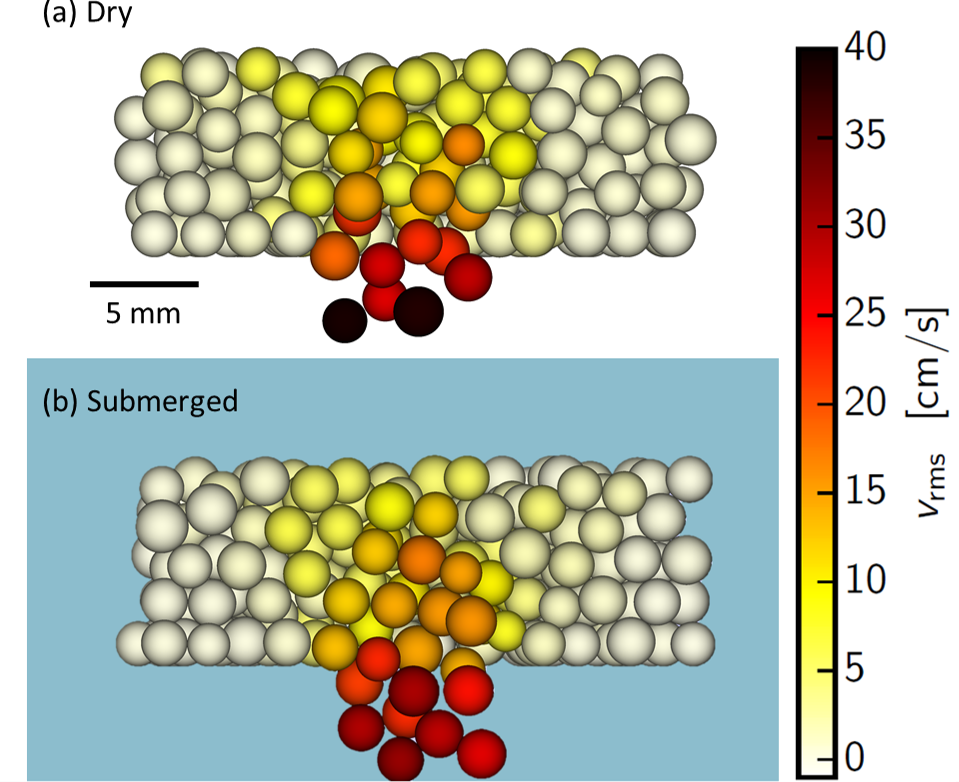
\includegraphics[width=\columnwidth]{fig1-snapshot_sim.png}
%DIFDELCMD < \caption{%DIFDELCMD < \label{fig1}%%%
Snapshot of the simulation close from the orifice shows the localized particle velocities. Here, the 3D cylinder is visualized at the center plane. The dry simulation with particles in vacuum (a) has a lower packing fraction than the submerged case with water as interstitial medium (b). In the vacuum system, the flux is fully driven by gravity pulling the particles out from the hopper. In the submerged case in addition to gravity the particle flux is driven by the fluid pushing the particles. Due to this, the particle volume fraction at the exit is higher in the submerged case (b) compared to vacuum (a) as is visually evident.
%DIFDELCMD < \end{figure}
%DIFDELCMD < %%%
\DIFdelend 

The 3D hopper flow, shown in Fig.~\ref{fig1}, is a well studied model case of grain flow \cite{Thomas2016,Wilson2014,Thomas2015}, partly due to \DIFdelbegin \DIFdel{its seeming simplicity}\DIFdelend \DIFaddbegin \DIFadd{the fact that the geometry is simple allowing for easy implementation for the experimentalists}\DIFaddend , but also due to its importance in practical applications, from simple silos in farms to complex pharmaceutical factories. Even in a \DIFdelbegin \DIFdel{simple hopper scenario}\DIFdelend \DIFaddbegin \DIFadd{hopper flow}\DIFaddend , all three granular phases exist\DIFdelbegin \DIFdel{, and there is }\DIFdelend \DIFaddbegin \DIFadd{: }\DIFaddend the gas phase outside the hopper\DIFdelbegin \DIFdel{; }\DIFdelend \DIFaddbegin \DIFadd{, the solid phase }\DIFaddend near the hopper boundaries\DIFdelbegin \DIFdel{the grains are in the bulk or solid phase, while above the orifice, there must be a }\DIFdelend \DIFaddbegin \DIFadd{, and the }\DIFaddend yielded (fluid) phase \DIFaddbegin \DIFadd{directly above the orifice }\DIFaddend enabling the flow.
%DIF >  figure 1
\DIFaddbegin \begin{figure}[!th]
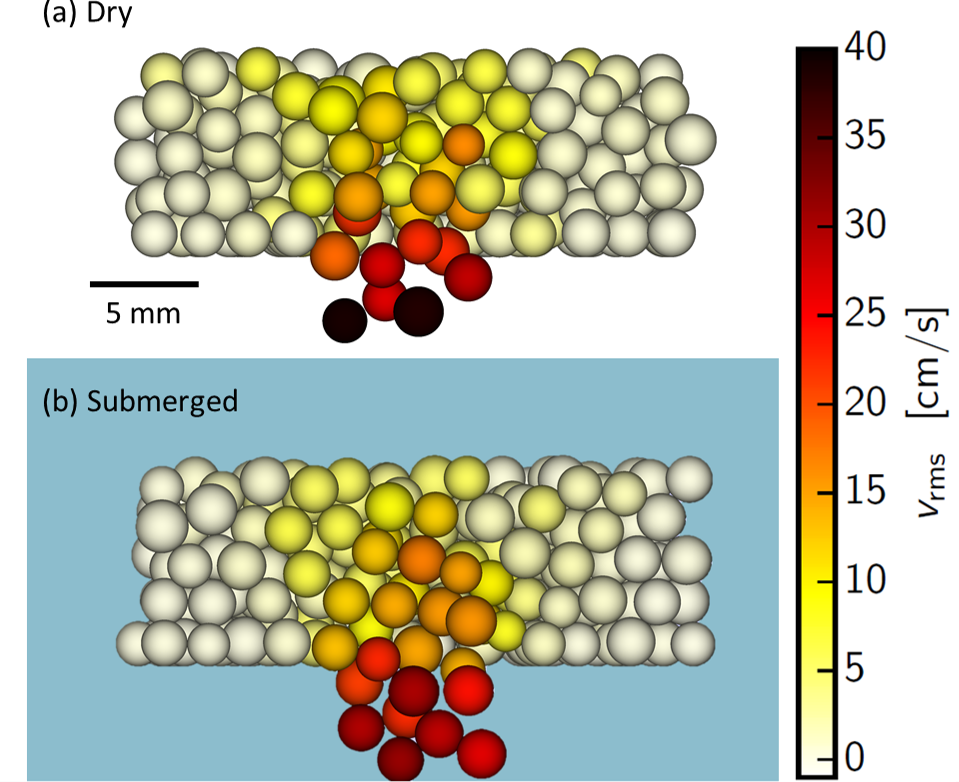
\includegraphics[width=0.97\columnwidth]{fig1-snapshot_sim.png}
\caption{\label{fig1}Snapshot of the simulation close from the orifice shows the localized particle velocities. Here, the 3D cylinder is visualized at the center plane.  In the vacuum system, the flux is fully driven by gravity pulling the particles out from the hopper. In the submerged case in addition to gravity the particle flux is driven by the fluid pushing the particles. Due to this, the particle volume fraction at the exit is higher in the submerged case (b) compared to vacuum (a) as is visually evident.}
\end{figure}
\DIFaddend 


Numerous studies have shown that in a dry hopper, the outflow 
of the granular particles follows the Beverloo equation~\DIFdelbegin \DIFdel{\mbox{%DIFAUXCMD
\cite{Beverloo1961,Madrid2016Arx,AshourSM17}}\hspace{0pt}%DIFAUXCMD
. 
That is, the outward flux of 
grains }\DIFdelend \DIFaddbegin \DIFadd{\mbox{%DIFAUXCMD
\cite{Beverloo1961,Madrid2017EPJ,AshourSM17}}\hspace{0pt}%DIFAUXCMD
, which
states that the grain outward flux }\DIFaddend remains constant in time \DIFdelbegin \DIFdel{, }\DIFdelend until the hopper \DIFdelbegin \DIFdel{runs out of grains.
The grain liquid interaction culminates to three components: terminal velocity as well as Darcy and modified Beverloo equations. The Beverloo equation for }\DIFdelend \DIFaddbegin \DIFadd{empties.
The Beverloo equation for a }\DIFaddend dry case
%
\begin{equation}
W_{dry} = C \rho \sqrt{g}(D-kd)^{(5/2)}
\end{equation}
%
describes the mass flow rate as a function of \DIFaddbegin \DIFadd{the }\DIFaddend density $\rho$, gravity $g$ as well as particle $d$ and orifice $D$ diameters.
The term $D-kd$ illustrates the empty annulus where the particles partially reduce the size of the orifice through constant $k$. 
The exponent 5/2 can be derived through the so called free fall theorem 
that essentially says that the flow rate is proportional to the particle 
velocity as if it would \DIFdelbegin \DIFdel{fall of a dome covering }\DIFdelend \DIFaddbegin \DIFadd{freely fall from granular bulk forming a semisphere above }\DIFaddend the orifice 
\cite{Tian2015,Janda2012,Mankoc2007}. 
The geometry then dictates the exponent 5/2. 
\DIFdelbegin %DIFDELCMD < 

%DIFDELCMD < %%%
\DIFdel{Recently the Beverloo equation is adapted and simplified to the liquid case \mbox{%DIFAUXCMD
\cite{Wilson2014} 
}\hspace{0pt}%DIFAUXCMD
%DIF < 
}\begin{displaymath}
	\DIFdel{W = C\rho v_t d^2 (D/d - k)^2, %DIFDELCMD < \label{eq:modified-beverloo}%%%
}\end{displaymath}   
%DIFAUXCMD
%DIF < 
%DIFDELCMD < \noindent %%%
\DIFdel{where the acceleration due gravity in fixed distance is replaced by terminal velocity $v_t$ in a liquid. It is important to note that the flow decreases to zero when the ratio $D/d$ approaches $k$. The $C=0.4$ and $k=2.4$ are the empirical fit parameters in a submerged case \mbox{%DIFAUXCMD
\cite{Wilson2014,koivistoSubmitted}}\hspace{0pt}%DIFAUXCMD
.
}%DIFDELCMD < 

%DIFDELCMD < %%%
\DIFdelend The Beverloo equation \DIFaddbegin \DIFadd{has the drawback that it }\DIFaddend only considers the dimensions of the grains and the orifice but not the properties of the interstitial medium, such as viscosity or drag.
\DIFaddbegin 


\DIFaddend Some studies have considered the role of air as an interstitial 
medium \cite{Yuu2011Mat}. There are simulations and experiments that 
show non-trivial flow patterns of air \DIFdelbegin \DIFdel{when particles move, starting 
from }\DIFdelend \DIFaddbegin \DIFadd{due to particle motion, showing 
}\DIFaddend oscillations \cite{WuX.L.Maloy1993,Bertho2002} and \DIFdelbegin \DIFdel{steady state 
turbulent like flows }\DIFdelend \DIFaddbegin \DIFadd{flows resembling  
turbulence }\DIFaddend \cite{Hilton2011}. This movement of gas \DIFdelbegin \DIFdel{like 
medium }\DIFdelend affects the flow of 
grains by creating pressure gradients and drag. 
These effects are in this case minor, since the drag caused
by air is rather modest.


When the grains are embedded in a liquid, whose viscosity is orders of magnitude larger compared to that of air,
the effect of interstitial medium is expectedly more pronounced \cite{koivistoSubmitted}.
\DIFdelbegin \DIFdel{There, the flow rate of grains actually increases in time, i.
e.  
~surges \mbox{%DIFAUXCMD
\cite{Wilson2014}}\hspace{0pt}%DIFAUXCMD
. Compared }\DIFdelend \DIFaddbegin \DIFadd{Recently the Beverloo equation was adapted and simplified to include the interstitial liquid \mbox{%DIFAUXCMD
\cite{Wilson2014} 
}\hspace{0pt}%DIFAUXCMD
%DIF > 
}\begin{equation}
	\DIFadd{W_{go} = C\rho v_t d^2 (D/d - k)^2 \label{eq:modified-beverloo}.
}\end{equation}   
%DIF > 
\noindent \DIFadd{Here the acceleration due to gravity in fixed distance is replaced by terminal velocity $v_t$ of a single particle in a liquid. 
Here, we mark the flow rate $W$ with a subindex $go$ to emphasize that this is the reference flow rate for infinitely high packings with passive fluid flow at the steady state \mbox{%DIFAUXCMD
\cite{koivistoSubmitted}}\hspace{0pt}%DIFAUXCMD
.
The empirical fit parameters are $C=0.4$ and $k=2.4$ \mbox{%DIFAUXCMD
\cite{Wilson2014,koivistoSubmitted}}\hspace{0pt}%DIFAUXCMD
.  
In addition, as opposed }\DIFaddend to a Newtonian fluid running out of a bucket\DIFdelbegin \DIFdel{this behaves exactly the opposite; there the }\DIFdelend \DIFaddbegin \DIFadd{, where the }\DIFaddend flow rate decreases as the \DIFdelbegin \DIFdel{water runs out. }\DIFdelend \DIFaddbegin \DIFadd{fluid runs out, in the submerged granular system the flow rate of grains is observed to increase in time, i.e.~surges \mbox{%DIFAUXCMD
\cite{Wilson2014}}\hspace{0pt}%DIFAUXCMD
. }\DIFaddend In this submerged granular flow, the complexity of the problem rises from the fluid-particle interactions. As in the dry hopper scenario, the driving force of the system is the particle flow created by gravity. However, here the motion of the particles additionally creates fluid flow that disturbs the particle trajectories. This feedback loop between fluid and particles presumably increases the driving pressure of grains as they run out. A simple analytical model taking this into account is already shown in \DIFdelbegin \DIFdel{Ref.}\DIFdelend \DIFaddbegin \DIFadd{Reference}\DIFaddend ~\cite{koivistoSubmitted}.



%DIF < Loppuun 
\DIFdelbegin \DIFdel{In this paper we show that one can successfully capture both qualitatively and quantitatively this counter intuitive behavior arising in a submerged granular hopper flow using coupled discrete element model (DEM) for the particle dynamics and computational fluid dynamics (CFD). While the particle trajectories and interactions are computed explicitly in the DEM-implementation, the fluid flow is modeled on a continuum level by the CFD approach. This is fundamentally different from the inertial $\mu(I_v)$-model where the granular media and the interstitial fluid is treated as a single continuum \mbox{%DIFAUXCMD
\cite{Boyer11PRL}}\hspace{0pt}%DIFAUXCMD
.
%DIF < \NOTEC{$\mu(I)$-model should not be compared directly with a suspension, but $\mu(I_v)$-model can. Can we change argument from I to Iv? Or, add a reference to Boyer's paper to clarify that we really mean the suspension model not the granular model?}. Furthermore, we focus on the flow of spherical particles and how it changes via modifications in the properties of the interstitial medium and inter-particle friction. 
%DIF < Write about the key point:
}%DIFDELCMD < 

%DIFDELCMD < %%%
\DIFdelend The article is organized as follows: It starts by introducing the reader to our Methods, giving the details of both the experiments and the simulations. Then in the section Results we describe the main findings, showing that the features observed in experiments are captured by the simulations. Once the validity of the simulation is confirmed, the values of grain-grain friction is \DIFdelbegin \DIFdel{swept using simulations.
%DIF < \NOTEC{interparicle is used here, but grain-grain below. Should pick one.}. 
}\DIFdelend \DIFaddbegin \DIFadd{varied in the simulations.
}\DIFaddend The article finishes with Conclusions, where we discuss the results, and give the readers a short overlook to future research.

\section{Methods}

Here, we study both the dry and submerged granular hopper flows.
In the simulations, we assume that we can model the dry case without 
the interstitial fluid (no CFD), since  air viscosity and density are 
negligible.
In contrast, the submerged granular flow comprises two distinct 
phases (granular particles and liquid) that interact by various forces 
and have to be modeled concurrently. 
The approach adopted here is to model the liquid phase on a continuum 
level and the granular phase as discrete particles. Specifically, the 
fluid phase is modeled by the Computational Fluid Dynamics (CFD) 
method~\cite{ferziger2012computational}, which utilizes the Finite Volume 
Method (FVM) for discretizing the Navier-Stokes in the problem domain. 
The Discrete Element Method (DEM)~\cite{cundall1979discrete} is applied 
for the granular (particle) phase and each particle trajectory is 
integrated individually based on the interaction forces.

In the CFD framework, the modified Navier-Stokes equations (NSEs)
~\cite{anderson1967fluid}, physically implying the conservation of mass 
and momentum, are discretized and solved to yield the relevant quantities, 
such as the local fluid velocity and pressure fields.
\DIFdelbegin \DIFdel{The modified NSEs 
(here, Eqs. (23) and (40) in Ref.
~\mbox{%DIFAUXCMD
\cite{anderson1967fluid}}\hspace{0pt}%DIFAUXCMD
) }\DIFdelend \DIFaddbegin \DIFadd{For an incompressible fluid, these read~\mbox{%DIFAUXCMD
\cite{zhou2010discrete}
}\hspace{0pt}%DIFAUXCMD
}\begin{equation}
\DIFadd{\begin{split}
 \frac{\partial \epsilon_f}{\partial t} + \nabla \cdot \left( \epsilon_f \mathbf{u} \right) &= 0, \\
 \rho_f \epsilon_f \left[ \frac{\partial \mathbf{u}}{\partial t} + \nabla \cdot \left( \mathbf{u}\mathbf{u} \right) \right] &=
 \nabla \cdot \tau -n\mathbf{f}_i + \rho_f \epsilon_f \mathbf{g} ,
\end{split}
}\end{equation}
\DIFadd{where $\epsilon_f$ is the fluid volume fraction, $\mathbf{u}$ is the fluid velocity, $\rho_f$ is the fluid density,
$\tau$ is the Cauchy stress tensor and $\mathbf{g}$ is the gravity term.
Additionally, these modified NSEs 
}\DIFaddend include the 
particle-fluid interaction term \DIFaddbegin \DIFadd{($n\mathbf{f}_i$)}\DIFaddend , that contains the sum of the appropriate 
interaction forces \DIFaddbegin \DIFadd{over a number of particle $n$}\DIFaddend , such as the \DIFaddbegin \DIFadd{(Di Felice) }\DIFaddend drag force \cite{DiFelice1994}, buoyancy, 
pressure gradient forces and the imposed shear stress~\cite{zhu2007discrete}. 
This term is also present in the DEM scheme, where it is included in the 
Newton's 2nd law which is formulated and solved for each particle.
\DIFdelbegin \DIFdel{This }\DIFdelend \DIFaddbegin \DIFadd{More specifically, the equations of motion in DEM are~\mbox{%DIFAUXCMD
\cite{zhou2010discrete}
}\hspace{0pt}%DIFAUXCMD
}\begin{equation}
\DIFadd{\begin{split}
 m_i\frac{\partial \mathbf{v}}{\partial t} &= \mathbf{f}_i + \sum_{j=1}^{n_c} \left(\mathbf{f}_{c, ij} + \mathbf{f}_{d, ij} \right) + m_i\mathbf{g} \\
 I_i\frac{\partial \mathbf{\omega}_i}{\partial t} &= \sum_{j=1}^{n_c} \left(\mathbf{M}_{t, ij} + \mathbf{M}_{r, ij} \right) ,
\end{split}
 }\end{equation}
\DIFadd{where $m_i$ is the mass of particle $i$, $\mathbf{v}$ is the velocity of the said particle, $\mathbf{f}_{c, ij}$ and $\mathbf{f}_{d, ij}$ describe the elastic deformation
and viscous energy dissipation of the particle while in contact with particle $j$. Further, $I_i$ is the moment of inertia of the particle while $\mathbf{M}_{t, ij}$ and
$\mathbf{M}_{r, ij}$ describe the torque generated by tangential forces in a collision and rolling friction, respectively. Here, we have set the rolling friction to zero.
}

\DIFadd{The presented }\DIFaddend coupling scheme has the inherent advantage of providing an accurate 
description of both the fluid and the particle phase at a reasonable 
computational expense~\cite{zhu2007discrete}.
\DIFdelbegin %DIFDELCMD < 

%DIFDELCMD < %%%
\DIFdel{The }\DIFdelend \DIFaddbegin \DIFadd{Furthermore, the }\DIFaddend CFD-DEM coupling is realized in a readily implemented software called CFDEM project which combines
the OpenFOAM CFD-library with a DEM solver (LIGGGHTS~\cite{kloss2012models}), providing the user  extensive control over the simulation particulars and more importantly, the NSEs and fluid-particle interaction models~\cite{zhou2010discrete}. The implementation also grants efficient CPU parallel execution via the Message Passing Interface (MPI).

The material parameters used in the numerical method are obtained, where possible, from the experiments or utilizing textbook values.
In the experiments, there are three types of grains, while in the simulations only the largest one is used. The grains are technical quality soda lime silica glass beads with $d=0.2\pm0.01$ cm (A-205),  $d=0.1\pm0.01$ (A-100) and $d=0.05\pm0.005$ (P-230) in diameter from Potters Industries. Their density is $\rho=2.54 \pm 0.01~\mathrm{g/cm^3}$ measured using the Archimedes method by sinking the beads in liquid and measuring the weight of the grains and fluid volume displacement. 
\DIFaddbegin \DIFadd{These values of the grain properties were set in the simulations to match the experimental values.
}\DIFaddend The simulations additionally require knowledge of the elastic (Young's and shear) moduli, and the friction and restitution coefficients.
The typical values for Young's and shear moduli of glass beads tabulated in textbooks are $E=72$ GPa and $G=30$ GPa, respectively.
These give the Poisson's ratio of $p = E/(2G) - 1 = 0.2$. 
\DIFdelbegin \DIFdel{These values of the grain properties were set }\DIFdelend \DIFaddbegin \DIFadd{The parameters used }\DIFaddend in the simulations \DIFdelbegin \DIFdel{to match the experimental values}\DIFdelend \DIFaddbegin \DIFadd{are summarized in Tab.~\ref{tab:properties}. 
It has been shown that a lower value of Young's modulus can be used without affecting the results \mbox{%DIFAUXCMD
\cite{Lommen2014Par} }\hspace{0pt}%DIFAUXCMD
and this is also what we have observed while benchmarking our algorithm}\DIFaddend .

%DIF < figure 2
\DIFdelbegin %DIFDELCMD < \begin{figure}
%DIFDELCMD < 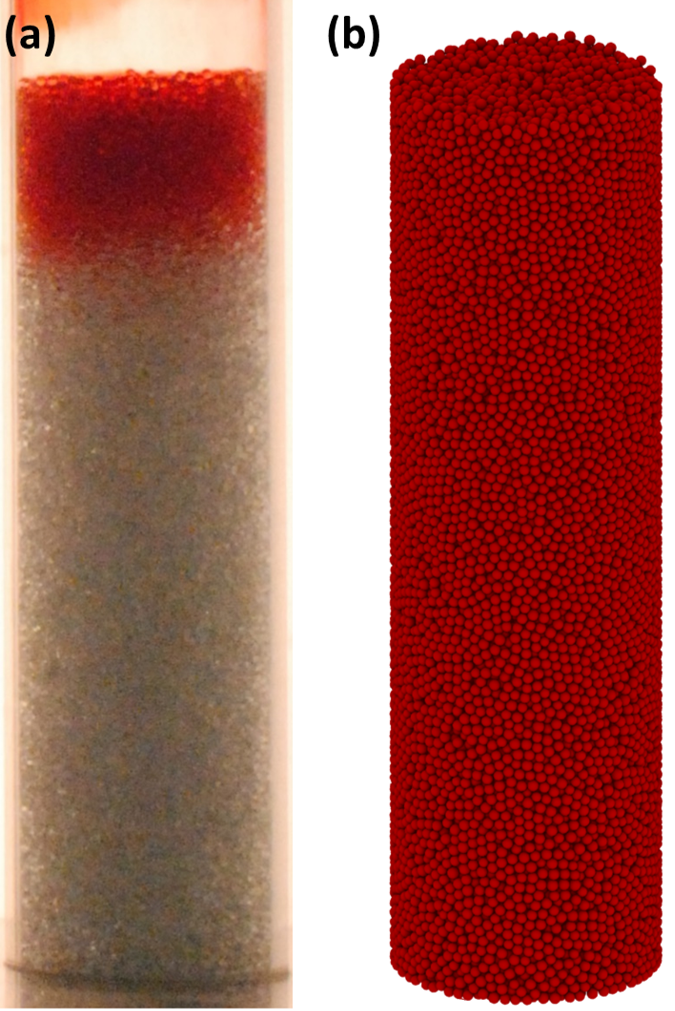
\includegraphics[width=\columnwidth]{fig2-snapshot_exp_sim.png}
%DIFDELCMD < \caption{Experimental (a) and numerical (b) geometries are the same; The orifice diameter is $D=1.0$ cm, particle diameter $d=0.2$ cm and hopper diameter $D_h=5.0$ cm. The red dye injected on top of the grains in the experiments (a) is visualizing the fluid flow. The grains are transparent glass but appear albescent.
%DIFDELCMD < \label{fig:Geometry}}
%DIFDELCMD < \end{figure}
%DIFDELCMD < %%%
\DIFdelend \DIFaddbegin \begin{table}[!b]
\caption{The values for the particle and fluid properties applied in the simulations and experiments. The more detailed technical information on the simulations is provided as  Supplementary Data 1. The values marked with star are textbook values.}\label{tab:properties}
\setlength{\extrarowheight}{2pt}
  \begin{tabular*}{0.5\textwidth}{@{\extracolsep{\fill}}lccccc}

 \hline
 & & &	simulation		& experiment \\
    \hline
~~~Granular particles~~~	&\\[2pt]
\hline
Density of glass 				& $\rho$			& $\mathrm{[g/cm^3]}$		& 2.5 					& 2.54	~\\
Young's Modulus 			& $E$				& $\mathrm{[GPa]}$			&	0.025				& 72*	~\\
Shear Modulus 				& $G$ 				& $\mathrm{[GPa]}$			& \textendash	& 30*	~\\
Poisson's ratio					& $p$				&														& 0.2						& 0.2	*	~\\ 
Restitution coefficient	& $\alpha$		&														& 0.9   					& \textendash ~\\
Timestep (DEM) 			& $dt$				& $[\mu\mathrm{s}]$			&	5.0				& --	~\\
\hline
~~~Fluid~~~	&\\[2pt]
\hline
Density of water				& $\rho_f$		& $\mathrm{[g/cm^3]}$			& 1.0 				& 1.0* ~\\
Viscosity								& $\eta$			& $\mathrm{[mPa\cdot s]}$	& 1.0					& 1.0* ~\\
Timestep (CFD)								& $dt$			& $[\mu\mathrm{s}]$	& 50.0					& -- ~\\
Coupling interval								& $d\tau$			& $[\mu\mathrm{s}]$	& 500.0					& -- ~\\
\hline
\end{tabular*}

\end{table}
\DIFaddend 

%DIF < \FloatBarrier
\DIFdelbegin %DIFDELCMD < 

%DIFDELCMD < %%%
\DIFdelend The friction and restitution coefficients, describing the dissipation of the grain-grain contacts and collisions, are the 
remaining parameters required to perform DEM simulations. Measurement of either of these for glass beads is impractical as it requires to estimate the dissipated energy in a dense granular flow. A textbook value for sliding of wet glass surfaces is around $\mu=0.1$, which can be taken as a starting point for the simulations. 
A sensible value for the restitution coefficient of hard-sphere-like glass beads is $\alpha=0.9$. For instance, in similar dry simulations involving softer grains, the restitution coefficient of $\alpha=0.8$ has been used \cite{SchwartzGM12}. 

%DIF < \subsection{water}
\DIFdelbegin %DIFDELCMD < 

%DIFDELCMD < %%%
\DIFdel{In the }\DIFdelend \DIFaddbegin \DIFadd{In the experimental }\DIFaddend setup, the liquid phase consists of filtered tap water at $T=22~\degree C$ temperature with the well known textbook values 
for viscosity $\eta = 1.0$~mPa$\cdot$s and density $\rho_f=1.00~\mathrm{g/cm^3}$. Accordingly, these values were used in the 
simulations, with the further assumption of laminar flow conditions. 
Laminar flow can be safely assumed owing to the fact 
that the flow rates remain rather modest being purely 
driven by the release of the grains' potential energy.
In practice the hopper is submerged in a large fish tank. There are 
no water -- air interfaces. The experiment is totally under water. 
The scale is above the water level, measuring the weight of 
the remaining beads in the hopper. 
The hopper is a flat 
bottomed cylindrical tube made of transparent polycarbonate with $D_h = 5.0$~cm diameter. 
The orifice is a circular hole ($D=1.0$~cm) with 1~mm vertical walls that expand in 45-degree bevel cut at the center of the aluminum bottom. 
The experimental setup is described in detail in Refs.~\cite{koivistoSubmitted,koivisto2017PRE} and their supplemental material.

%DIF < \subsection{methods and devices}
\DIFdelbegin %DIFDELCMD < 

%DIFDELCMD < %%%
%DIF < dry and submerged. settling, scale, etc
%DIFDELCMD < 

%DIFDELCMD < %%%
%DIF < In the submerged case there are no water - air interfaces; the experiment is totally under water.
%DIFDELCMD < 

%DIFDELCMD < %%%
\DIFdelend %DIF > figure 2
\DIFaddbegin \begin{figure}
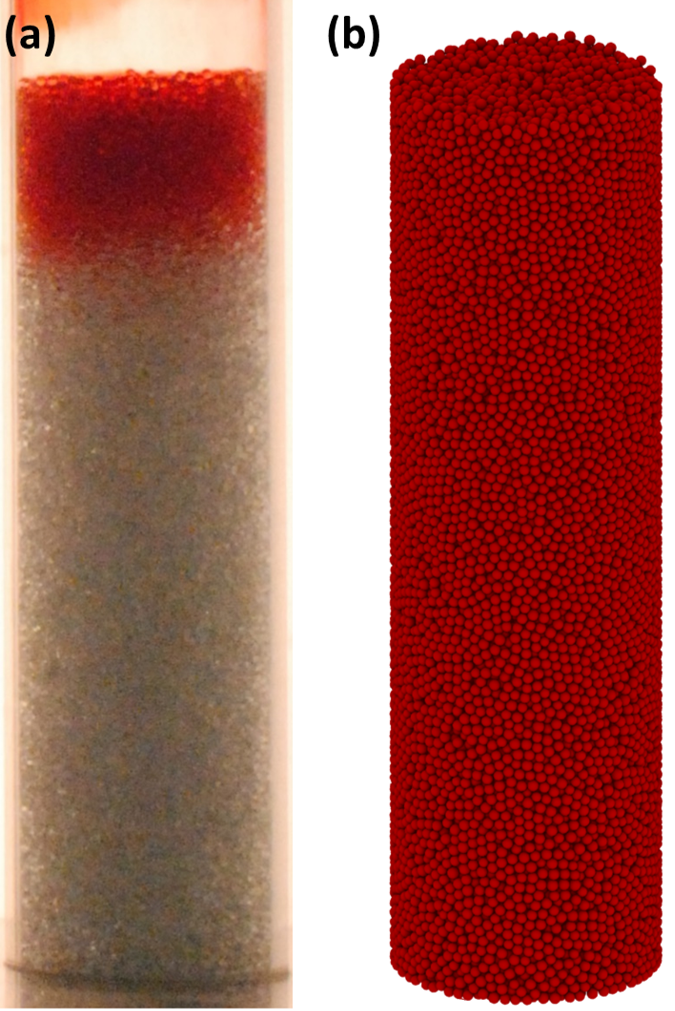
\includegraphics[width=\columnwidth]{fig2-snapshot_exp_sim.png}
\caption{Experimental (a) and numerical (b) geometries are the same; The orifice diameter is $D=1.0$ cm, particle diameter $d=0.2$ cm and hopper diameter $D_h=5.0$ cm. The red dye injected on top of the grains in the experiments (a) is visualizing the fluid flow. The grains are transparent glass but appear albescent.
\label{fig:Geometry}}
\end{figure}
%DIF > 
\DIFaddend Fig.~\ref{fig:Geometry} displays both the experimental 3D hopper (a) as well as its simulation counterpart (b). The initial state of the \DIFaddbegin \DIFadd{experimental }\DIFaddend hopper contains 50~\% more beads than shown in Fig.~\ref{fig:Geometry}(a). The red dye at the top was injected on top of the granular pile before the experiment and it propagates through the hopper faster than the grains can exit the system. (See the supplementary videos 1 and 2 which illustrate this process.)

The geometry is the same in the simulations and experiments, with very few exceptions. The initial filling height is smaller in the simulations, 
the hopper walls possess no thickness and have the same friction coefficient as the grains. The CFD simulation domain is divided into 1.5 million cells. The grid size gradually decreases near the hopper boundaries to ensure the quality of the solution in those areas. The meshing is realized applying the snappyHexMesh-tool embedded in the OpenFOAM software~\cite{openfoamdoc}.
%


In the simulations, the hopper flow is generated by first filling the hopper with the granular medium by pouring 
randomly the particles above the hopper top while the orifice remains closed. Then, once a sufficient filling height $h$ is
obtained, the granular packing is allowed to relax without the fluid for 0.5~seconds. At this point, the selection between the 
vacuum and submerged cases is made. In the vacuum case the orifice is opened, and the simulation is continued.
In the submerged case, the coupled CFD-DEM simulation is initiated and the orifice is opened. 


\section{Results}

Motivated by the large computational cost of the prescribed numerical simulations, we revisit our earlier experimental findings with a new perspective.
The goal is to find a good compromise between having a long enough experiment with good surge per noise ratio (improves by reducing the particle size) and the computational burden (decreases with increasing particle size). The total particle number that can be handled with reasonable computational cost can be reached using the  average grain diameter of $d=0.2$~cm. 
Our main concern is the impact of the particle size on the surge. 
Hence, we start by comparing the earlier studied systems  having $d=0.05$~cm and $d=0.1$~cm \DIFaddbegin \DIFadd{\mbox{%DIFAUXCMD
\cite{koivistoSubmitted} }\hspace{0pt}%DIFAUXCMD
}\DIFaddend to the new system with $d=0.2$~cm. For this purpose, we observe the flow rate and compute selected dimensionless numbers characterizing the systems

%DIF < We begin the results section by revisiting and expanding experimental 
%DIF < findings with a new perspective. 
%DIF < This is motivated by heavy computational cost of the numerical simulations.
%DIF < Currently, we must find a
%DIF < compromise between a reduced number of particles dictated by simulations, but still enough to produce a granular flow slow and long enough for good experimental accuracy. 
%DIF < We resolve this problem by extending the experiments from the
%DIF < $d=0.05$ cm and $d=0.1$ cm  used in earlier studies to $d=0.2$ cm particles thus reducing the particle 
%DIF < number by a factor of 8 to a feasible level.
%DIF < Hence, we first take an experimental look at the effect of particle size to the surge, flow rate
%DIF < and a selected dimensionless numbers characterizing the system.
\DIFdelbegin %DIFDELCMD < \begin{figure}[!t]
%DIFDELCMD < 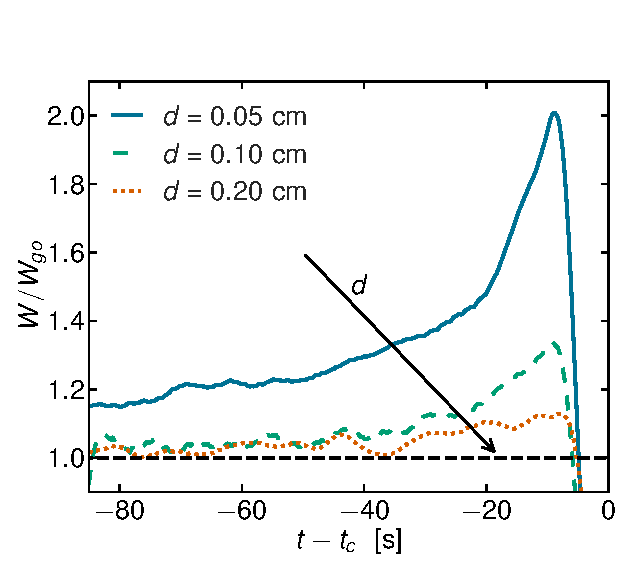
\includegraphics[width=\columnwidth]{fig3-surge.pdf}\\
%DIFDELCMD < %\vspace{-2cm}
%DIFDELCMD < %\includegraphics[width=\columnwidth]{fig3/figure_xx_qgo_vs_d.pdf}
%DIFDELCMD <  

%DIFDELCMD < \caption{The relative mass flow rate of hopper for three different particle sizes. The flow rate $W$ is normed with the flow rate $W_{80}$ that is the flow rate 80 seconds before the end. We find that the surge, the acceleration at the end decreases as particle size increases.
%DIFDELCMD < \label{fig:surge}}
%DIFDELCMD < \end{figure}
%DIFDELCMD < %%%
\DIFdelend \DIFaddbegin \begin{figure}[!t]
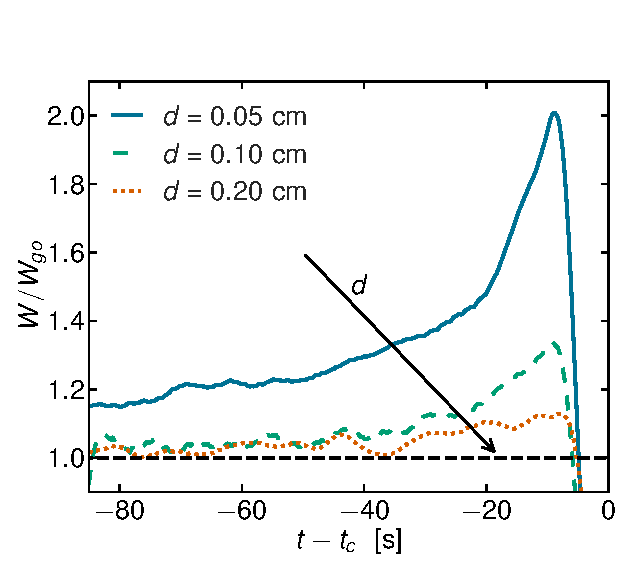
\includegraphics[width=\columnwidth]{fig3-surge.pdf}\\

\caption{The relative mass flow rate of hopper for three different particle sizes. 
The flow rate $W$ is normed with the flow rate $W_{go}$ depicted with dashed line that is the asymptotic reference flow rate for infinitely high packings. 
We find that the surge, the acceleration at the end decreases as particle size increases.
\label{fig:surge}}
\end{figure}
\DIFaddend %
Fig.~\ref{fig:surge} shows the relative flow rate against time 
$t-t_{c}$, where the $t_{c}$ is the time when the flow stops. 
The flow rate $W$ is obtained by differentiating the mass time series of the 
scale by fitting a $2^{\mathrm{nd}}$ degree polynomial in a 2 second 
Gaussian window similarly to Ref.~\cite{koivistoSubmitted}.
As we are interested on the surge and dynamic effects we scale the data by the \DIFdelbegin \DIFdel{flow rate at $t=t_c-80$ s}\DIFdelend \DIFaddbegin \DIFadd{reference flow rate obtained from the modified Beverloo equation (\ref{eq:modified-beverloo})}\DIFaddend . 
This operation allows us to compare the surge between the systems having different particle sizes.

The surge, the increase of flow rate $W$ with respect to the asymptotic value 
$W_{go}$ decreases with increasing particle size as highlighted by the black arrow in Fig.~\ref{fig:surge}. 
\DIFaddbegin \DIFadd{Also, the lifetime of the surge decreases when particle size increases which makes the comparison to simulations easier for larger particles than the small ones.
}\DIFaddend The largest increase $W_{surge} = \mathrm{max}(W) - W_{go}$ is with 
$d=0.05$~cm particles and the smallest is with $d=0.2$~cm particles. 
This agrees with earlier findings as the surge term 
containing the fluid-grain coupling has $d$ dependence as \DIFdelbegin \DIFdel{$W\propto(D-kd)^2$ 
}\DIFdelend \DIFaddbegin \DIFadd{$W_{surge}\propto(D-kd)^2$ 
}\DIFaddend (after expanding $\alpha$ from the supplementary material in 
Ref.~\cite{koivistoSubmitted}). 
The surge $W_{surge}$ thus decreases when approaching the clogging region 
from below by increasing the particle size \DIFaddbegin \DIFadd{$d$}\DIFaddend . 
There is no flow, nor surge above the clogging region. 
We conclude that the large particles in our case approach to a limit where 
the granular aspect of the system starts to dominate. 
The inertia of the grains is too high for the fluid that there would be a 
large surge.
% 
\DIFaddbegin \begin{figure}[!t] % figure 4
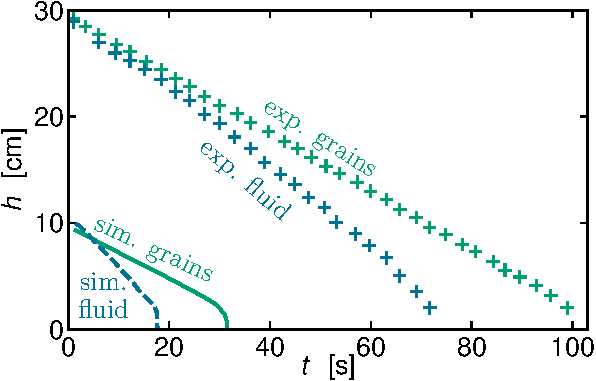
\includegraphics[width=\columnwidth]{fig4_fluid_is_faster.pdf}\\
\caption{The Fluid-is-Faster effect is illustrated by plotting the trajectories of tracer particles.
The green symbols represent the height of the granular column where the tracer particle is the highest particle at the side of the hopper. 
The blue symbols depict the lower edge of the dye.
In the simulations, the blue dashed curve represets the vertical position of a single point-like virtual fluid tracer obtained by post processing the continuum fluid field.
The green curve is the vertical position of one of the simulated grains.
The figure shows that the fluid has a greater superficial velocity in both cases.
The experiment and simulation are not directly comparable as the experimental values are averages while the simulation values are point-like measurements.
\label{fig:fluid_is_faster}}
\end{figure}
\DIFaddend 


\DIFdelbegin \DIFdel{Here, we would like to point }\DIFdelend \DIFaddbegin \DIFadd{Figure \ref{fig:fluid_is_faster} points }\DIFaddend out, that the superficial fluid velocity is faster than the grain velocity \cite{koivistoSubmitted}.
The fluid is faster and the inertia of the particles decreases the flow rate while the viscous component increases the flow.
This counterintuitive result is consistent with the earlier results 
\cite{koivistoSubmitted} and illustrated in supplementary video 1 with a 
layer of dye that propagates faster than the grains can exit. 
With small particles the fluid flow dominates the process and particles reflect to this.
The large particles have more momenta and inertia.
The fluid flow cannot affect the particle motion. \DIFdelbegin \DIFdel{The }\DIFdelend \DIFaddbegin \DIFadd{Then, 
the }\DIFaddend granular characteristics of the large particles dominate.

To obtain \DIFaddbegin \DIFadd{a }\DIFaddend more rigorous treatment we calculate dimensionless numbers that describe the flow.
Table \ref{tab:dimensionless} describes the dimensionless numbers of the system.
The Reynolds number $Re = \rho_f v_t d/\eta$ describes the ratio of inertial forces respect to viscous forces. 
It increases dramatically as the particle diameter increases ($Re \approx d^2$) indicating
the increase of granular behavior at the expense of fluid flow, provided the grain properties (grain-grain friction, and grain size distribution) remain the same.
%DIF < \NOTEC{The second half of this sentence seems a non sequitur. Flows can be very granular (highly interacting, dense, structure and friction matter) or not regardless of Reynolds number. Packing fraction and friction coefficient affect it more.   } 
At the same time, the drag coefficient decreases~\cite{Morrison2013Drag}, again, indicating 
the diminishing effect of fluid. Note that here we discuss only the laminar flow case.
%DIF < \NOTEC{This is also a non sequitur. Highly turbulent flows have a low drag coefficient, but that by no means indicates that the fluid is playing a minimal role. See e.g. turbulent driven ripples at beach.}.
Finally we calculate the inertial number that is the ratio of confining 
pressure and shear rate $I=\eta \dot{\gamma}/P$\DIFaddbegin \DIFadd{~~}\DIFaddend \cite{Houssais15NCO, Kamrin15SM}. 
The inertial number $I$ can be approximated by defining the shear rate 
$\dot{\gamma} = v_t/(D/2)$ as velocity difference at the orifice and an 
approximation of driving pressure $P = 1/2\;\rho_{e} v_t^2$
%DIF < \NOTEC{Need a schematic of pressure and shear rate near opening. Also, this is a fluid-like term. It's not clear this is the correct grain-grain pressure. I would argue the pressure must scale like the submerged weight of grains, similar to \texttt{10.1103/PhysRevLett.109.068001}} %\verb|10.1103/PhysRevLett.109.068001| } 
as
%
\begin{equation}
 I 	= \eta \frac{\dot{\gamma}}{P} = \eta \frac{D}{\rho_{e}v_t}, 
\end{equation}
%
\noindent where the effective density $\rho_{e}$ is the buoyancy 
corrected density. 
The particle geometry at the orifice is illustrated in Fig.~\ref{fig:freefall}.
For small particles the inertial number is large, at the region where the 
dynamic effects already play a role. For large particles 
the inertial number decreases and the dynamic friction coefficient 
saturates (close) to static value \cite{Singh15NJP}.
This is seen as a lack of terminal surge as a constant dynamic friction
coefficient $\mu(I)$ indicates constant flow rate. 
Also, recently \cite{Trulsson16PRE} it has been numerically found that the ratio of frictional and viscous dissipation changes in submerged particle systems. Here, we are approaching the frictional regime from viscous regime by increasing the particle size leading to vanishing surge. 
%
\DIFdelbegin %DIFDELCMD < \begin{figure}[!t]
%DIFDELCMD < \centering
%DIFDELCMD < \includegraphics[width=0.7\columnwidth]{fig4-schematic_freefall.pdf}\\
%DIFDELCMD < %\vspace{-2cm}
%DIFDELCMD < %\includegraphics[width=\columnwidth]{fig3/figure_xx_qgo_vs_d.pdf}
%DIFDELCMD <  

%DIFDELCMD < \caption{Schematic illustration of the particles at the orfice of size $D$ accelerating from rest (orange) to terminal velocity (green) due to gravity and thus creating a shear rate and pressure.
%DIFDELCMD < \label{fig:freefall}}
%DIFDELCMD < \end{figure}
%DIFDELCMD < %%%
\DIFdelend \DIFaddbegin \begin{figure}[!t]
\centering
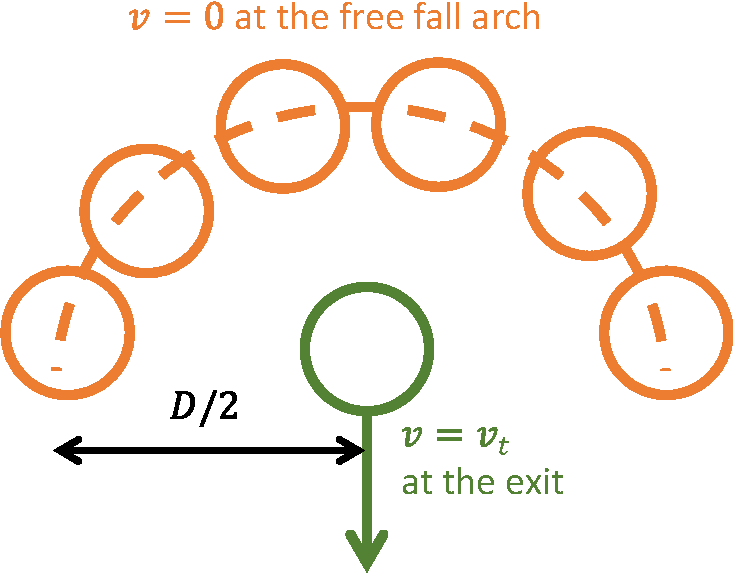
\includegraphics[width=0.7\columnwidth]{fig5-schematic_freefall.pdf}\\

\caption{Schematic illustration of the particles at the orifice of size $D$ accelerating from rest (orange) to terminal velocity (green) due to gravity and thus creating a shear.
\label{fig:freefall}}
\end{figure}
\DIFaddend 


\DIFdelbegin %DIFDELCMD < \begin{table}[!b]
%DIFDELCMD < \caption{Dismensionless numbers describing the system. All numbers 
%DIFDELCMD < indicate that the effect of fluid as the dynamic viscous component is 
%DIFDELCMD < decreasing.}%DIFDELCMD < \label{tab:dimensionless}%%%
%DIFDELCMD < \setlength{\extrarowheight}{2pt}
%DIFDELCMD <   \begin{tabular*}{0.5\textwidth}{@{\extracolsep{\fill}}cccrr}
%DIFDELCMD <     \hline
%DIFDELCMD < $d~~\mathrm{[cm]}$~	& ~~~$Re$~~~ 	& ~~~$C_d$~~~	&\multicolumn{1}{c}{~$I$~ }\\[2pt]
%DIFDELCMD < \hline
%DIFDELCMD < 0.05				& 37						& 1.76		&~$34.0 \times 10^{-4}$~\\
%DIFDELCMD < 0.10				& 151						& 0.86		&~$17.0 \times 10^{-4}$~\\
%DIFDELCMD < 0.20				& 530						& 0.56  	&~$ 9.8 \times 10^{-4}$~\\   \hline
%DIFDELCMD <   \end{tabular*}
%DIFDELCMD < 

%DIFDELCMD < \begin{tabular}{cccrr}
%DIFDELCMD < 

%DIFDELCMD < \end{tabular}
%DIFDELCMD < \end{table}
%DIFDELCMD < %%%
\DIFdelend \DIFaddbegin \begin{table}[!b]
\caption{Dimensionless numbers characterizing the system are
 the Reynold's number ($Re$) and the inertial number $I$.
 }\label{tab:dimensionless}
\setlength{\extrarowheight}{2pt}
  \begin{tabular*}{0.5\textwidth}{@{\extracolsep{\fill}}cccrr}
    \hline
$d~~\mathrm{[cm]}$~	& ~~~$Re$~~~ 	& ~~~$C_d$~~~	&\multicolumn{1}{c}{~$I$~ }\\[2pt]
\hline
0.05				& 37						& 1.76		&~$34.0 \times 10^{-4}$~\\
0.10				& 151						& 0.86		&~$17.0 \times 10^{-4}$~\\
0.20				& 530						& 0.56  	&~$ 9.8 \times 10^{-4}$~\\   \hline
  \end{tabular*}

\begin{tabular}{cccrr}

\end{tabular}
\end{table}
\DIFaddend 

 

%DIF < %%%%%%%%%%%%%%%%%%%%%%%%%%%%%%%%%%%%%%%%%%%%%%%%%%%%%%%%%%%% 
 \DIFdelbegin %DIFDELCMD < 

%DIFDELCMD < %%%
%DIF < The effect of particle size to submerged reference flow rate (at $h=\infty$) is well captured by the modified Beverloo equation [Wilson, KoivistoPreprint]
%DIF < \begin{equation}
%DIF <   Q_{go}=C v_t d^2 (D/d - k)^2,
%DIF < \end{equation}
%DIF < where the dimensionless empirical constants are $C = 0.4$ and $k=2.4$. The $v_t$ is the terminal velocity of the particles in water and it depends on the particle size. For the d=\{0.05, 0.1, 0.2\} cm particles the terminal velocities are $v_t=\{7.5, 15.1, 26.5\}$ cm/s. The corresponding reference flow rates are $Q_{go}=\{2.1, 3.3, 2.9\}~\mathrm{cm^3/s}$. The mass flow is obtained by multiplying with the density $W_{go} = \rho Q_{go} = \{\}$.
%DIFDELCMD < 

%DIFDELCMD < %%%
\DIFdelend The experimental study extends the research to larger particles in order
to reduce the particle number to a sufficient level to enable numerical 
simulations. 
\DIFdelbegin \DIFdel{The effect of grain size to the hopper flow is depicted in 
Fig.~\ref{fig:surge}, which shows the remaining mass of grains in the hopper
and the mass flow rate, both as a function of time for two different 
particle diameters. 
}\DIFdelend Not only the flow rate, but also the surge at the end of the experiment, 
depends on the particle diameter. As we have a grasp of the experimental 
aspects of the particle size dependence of the surge, it is possible to 
pick the largest particle size $d=0.2$~cm as a representative case.


%DIF <  figure 4
\DIFdelbegin %DIFDELCMD < \begin{figure}[!t] 
%DIFDELCMD <  \includegraphics[width=\columnwidth]{fig5-m_vs_t.pdf}
%DIFDELCMD < \caption{(a) The mass of grains inside the hopper as a function of time for various values of friction coefficient $\mu$. For nearly frictionless case (green, $\mu=10^{-6}$) the flow rate (slope) is high and decreases as the grains flow out. This corresponds to what happens with a Newtonian fluid (dashed curve). For high friction case (red, $\mu=0.8$) the behavior is linear with constant flow rate and corresponds to the standard Beverloo case. (b) The mass of particles inside a hopper as a function of time similarly to Fig.~(a). For low friction coefficients the flow rate (slope) is decreasing similarly to the dry case. The insets show the magnification of the datasets near the end. }
%DIFDELCMD <  \label{fig:friction_dry} \label{fig:friction_sub}
%DIFDELCMD < \end{figure}
%DIFDELCMD < %%%
\DIFdelend \DIFaddbegin \begin{figure}[!t] % figure 6
 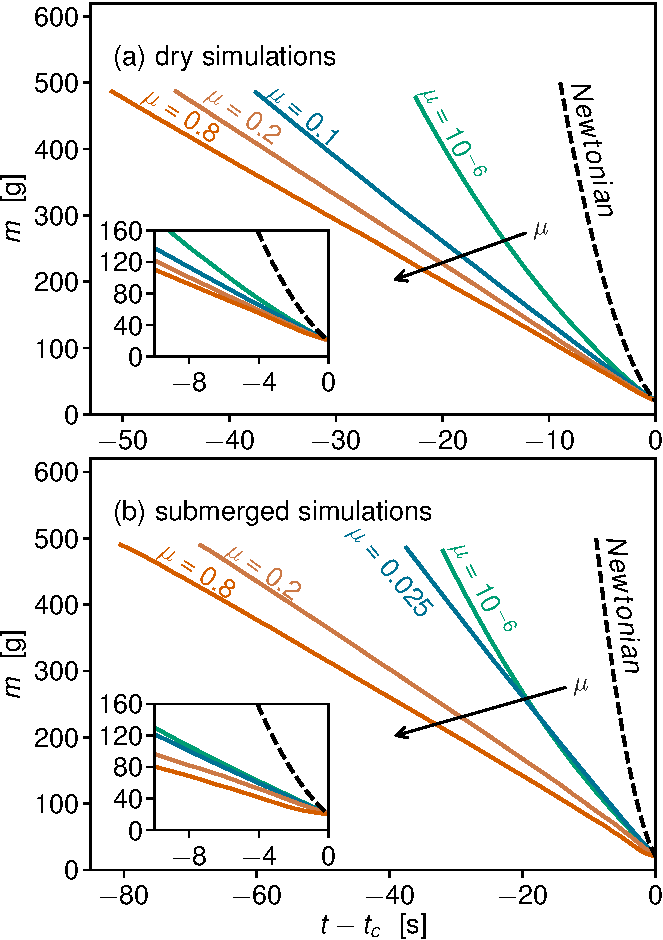
\includegraphics[width=\columnwidth]{fig6-m_vs_t.pdf}
\caption{(a) The mass of grains inside the hopper as a function of time for various values of friction coefficient $\mu$ for the dry system. For nearly frictionless case (green, $\mu=10^{-6}$) the flow rate (slope) is high and decreases as the grains flow out. This corresponds to what happens with a Newtonian fluid (dashed curve). For high friction case (red, $\mu=0.8$) the behavior is linear with constant flow rate and corresponds to the standard Beverloo equation. (b) The mass of particles inside a hopper as a function of time for the submerged system. For low friction coefficients the flow rate (slope) is decreasing similarly to the dry case. The insets show the magnification of the datasets near the end. }
 \label{fig:friction_dry} \label{fig:friction_sub}
\end{figure}
\DIFaddend %
%
In the simulations the low friction granular (cyan) and the Newtonian fluid (dashed black) cases in Fig.~\ref{fig:friction_dry}(a) are non-linear and therefore not described by the Beverloo equation (\ref{eq:modified-beverloo}). 
The inset in Fig.~\ref{fig:friction_dry}(a) shows the magnification of the data near the end of the experiment. This is to point out that there seems to be no acceleration in the flow rate. 
%DIF < The data does {\it not} dip just before the grains run out. 

Next, we repeat the simulation with parameters identical to the dry case with the exception that the grain-liquid coupling is enabled. Fig.~\ref{fig:friction_sub}(b) shows the mass in the hopper over $t-t_{c}$ as displayed earlier for the dry case in Fig.~\ref{fig:friction_dry}(a). The initial conditions, material parameters (except the friction coefficients), geometry, number of particles and even the initial particle locations are the same in each case. The largest difference is that the flow rates are significantly lower in the submerged cases. For instance, the simulation with the friction coefficient $\mu=0.8$ takes 52 seconds to empty 500 grams of grains in the dry case, while in the submerged case it takes 90 seconds. 

Additionally, there is an acceleration of the flow rate at the end of the simulation (Fig.~\ref{fig:friction_sub} insets). This is seen as separation of datasets and a slight downwards tilt in the data for the larger friction coefficients. Again, following the dry case, the low friction cases behave like Newtonian fluids without the acceleration. The contact friction of bulk granular materials is typically above $\mu=0.1$. For these values, we find a surge like feature in the submerged simulation, lacking from the dry case. As the only difference between the dry and submerged simulation is the inclusion of fluid, we conclude that the surge is due to the coupling between the liquid and grains.
%
\DIFdelbegin %DIFDELCMD < \begin{figure}[!t]
%DIFDELCMD < \includegraphics[width=\columnwidth]{fig6-wwo_vs_mu.pdf}
%DIFDELCMD < \caption{Flow rate at the beginning of the experiment versus friction coefficient for dry (red open circles) and submerged (blue filled squares) extracted from previous figures. The fit and functional form is purely empirical and used in finding the matching friction coefficient. The value of $W_{o,dry} = 9.5~\mathrm{g/s}$ and $W_{o,sub} = 6.1~\mathrm{g/s}$. The behavior appears to exponential in this narrow region. Here we anticipate the experimental results plotting the mass flow rate in dry experiments (red x) at $W_{dry} = 11.4~\mathrm{g/s}$ corresponding friction coefficient $\mu_{dry}=0.15$ in the simulations. Similarly, the mass flow rate in submerged experiments (blue +) is $W_{sub}=7.6~\mathrm{g/s}$ corresponding to friction coefficient $\mu_{sub} = 0.13$ in simulations.}\label{fig:q_vs_mu}
%DIFDELCMD < \end{figure}
%DIFDELCMD < %%%
\DIFdelend \DIFaddbegin \begin{figure}[!t]
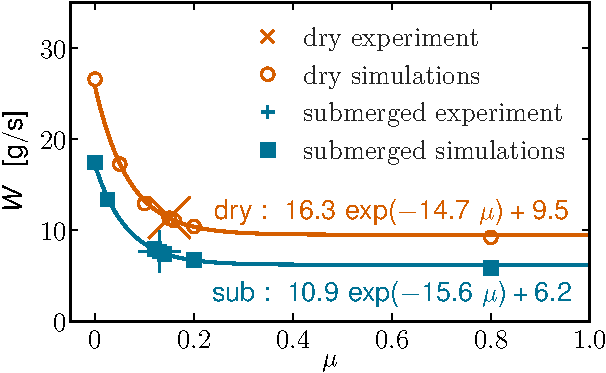
\includegraphics[width=\columnwidth]{fig7-wwo_vs_mu.pdf}
\caption{Flow rate at the beginning of the experiment versus friction coefficient for dry (red open circles) and submerged (blue filled squares) extracted from previous figures. The fit and functional form is purely empirical and used in finding the matching friction coefficient. The behavior appears to be exponential in this narrow region, highlighting how sensitive the flow rate is to the value of contact friction. Here we anticipate the experimental results by plotting the mass flow rate in dry experiments (red x) at $W_{dry} = 11.4~\mathrm{g/s}$ corresponding friction coefficient $\mu_{dry}=0.15$ in the simulations. Similarly, the mass flow rate in submerged experiments (blue +) is $W_{sub}=7.6~\mathrm{g/s}$ corresponding to friction coefficient $\mu_{sub} = 0.13$ in simulations.}\label{fig:q_vs_mu}
\end{figure}
\DIFaddend %
\DIFaddbegin {\DIFaddend In Fig.~\ref{fig:q_vs_mu}, we plot the simulated \DIFdelbegin \DIFdel{reduced flow rate $W-W_o$ }\DIFdelend \DIFaddbegin \DIFadd{flow rate $W$ }\DIFaddend with multiple values of the friction coefficient $\mu$, creating an empirical relation between the initial flow rate $W$ and the friction coefficient $\mu$. \DIFdelbegin \DIFdel{Here, $W_o$ is one of the fitting parameters. }\DIFdelend Based on this empirical relation we deduce the friction coefficient by matching the flow rates in the experiments at $m=300\ldots 400$~g. The red open circles correspond to the dry simulations  and the filled blue squares to the submerged simulations. The friction coefficients that reproduce the experiment are almost equal as $\mu_{dry}=0.15$ and $\mu_{sub}=0.13$ in the dry and submerged cases, respectively. The similarity in dry and submerged friction coefficient is also reported by Dijksman {\it et al.}~with acrylic beads in a rheometer \cite{DijksmanPRE10}. Note that here we refer to grain-grain friction \DIFdelbegin \DIFdel{$\mu$ }\DIFdelend whereas Dijksman {\it et al.}~refers to the  minimum friction coefficient $\mu_o$ at the quasi-static limit when inertial effects vanish $I\to 0$. The relation $\mu_o(\mu)$ is a non-trivial monotonic function that (to our knowledge) is only explored numerically \cite{Lemaitre09RHA,DaCruz05PRE,Trulsson16PRE}\DIFaddbegin \DIFadd{.}} \DIFaddend %Koval09PRE,Singh15NJP,Khamseh2015}.

%DIF < \NOTEC{This sentence is unnecessary and it draws attacks. Bulk granular friction differs from grain-grain friction quantitatively and also in functional dependence on other variables. It is simpler to quote the similarity of grain-grain friction submerged vs in fluid measurements directly. Dijksman himself did these measurements also.}
\DIFdelbegin %DIFDELCMD < 

%DIFDELCMD < %%%
%DIF < \subsection{Simulations match the experiments}
%DIFDELCMD < 

%DIFDELCMD < %%%
%DIF < In this section we show that the chosen simulation method matches the experiments both qualitatively and quantitatively. 
%DIFDELCMD < 

%DIFDELCMD < %%%
\DIFdelend \DIFaddbegin {\DIFaddend Fig.~\ref{fig:flow_rates} displays the mass \DIFaddbegin \DIFadd{of grains }\DIFaddend remaining in the hopper from both the experiments and the simulations with the friction coefficient set to the obtained values of $\mu_{dry}=0.15$ in the dry case and $\mu_{sub}=0.13$ in the submerged case. The submerged experiment is depicted in blue and the dry case in red color. The datasets are the result of a single run. The simulated and the experimental data are overlapping within the measurement accuracy. This lends credence to the computational approach applied in the work and specifically suggests that the coupled CFD-DEM model captures the quintessential features of the two-phase (submerged) hopper flow.\DIFaddbegin }

{\DIFadd{The nonlinear surge effect is highlighted in the insert with a blue area that is the difference between a linear fit and the experimental data before the flow rate slows down. 
The blue area is drawn to both cases, dry and submerged but is visible only in the submerged case.
This indicates that the constant flow rate predicted by the Beverloo law applies to the dry case but does not apply to the submerged case.  }}
\DIFaddend %
%DIF <  Figure 5: raw data
\DIFdelbegin %DIFDELCMD < \begin{figure}[!t]
%DIFDELCMD <  \includegraphics[width=\columnwidth]{fig7-m_vs_t-exp_sim.pdf}\\
%DIFDELCMD <  \caption{The raw data from the experiments and simulations show the difference between dry (red) and submerged (blue) case. The Linear fit depicted with solid line to the simulation data above $m = 200$~g matches the dry case perfectly until the grains run out. In submerged case the data takes a nose dive, surges, before the grains run out. Inset: the blue swath indicates a surge, difference between linear Beverloo behavior and measured data.}
%DIFDELCMD <  \label{fig:flow_rates}
%DIFDELCMD < \end{figure}
%DIFDELCMD < %%%
\DIFdelend \DIFaddbegin \begin{figure}[!t] % Figure 8: raw data
 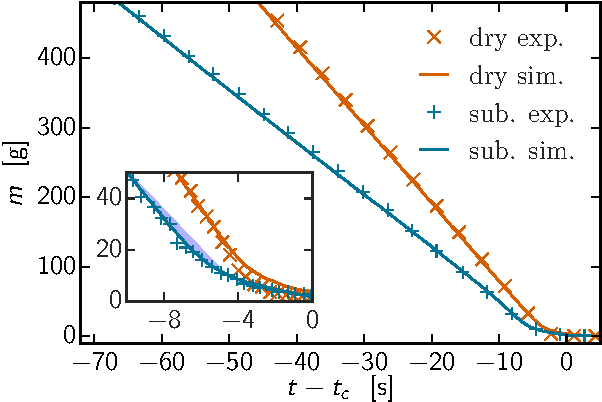
\includegraphics[width=\columnwidth]{fig8-m_vs_t-exp_sim.pdf}\\
 \caption{The raw data from the experiments and simulations show the difference between dry (red) and submerged (blue) case. The linear fit depicted with solid line to the simulation data above $m = 200$~g matches the dry case perfectly until the grains run out. In submerged case the data takes a nose dive, surges, before the grains run out. Inset: the blue area indicates a surge, the difference between linear Beverloo behavior and measured data.}
 \label{fig:flow_rates}
\end{figure}
\DIFaddend 

Fig.~\ref{fig:derivated_data} displays the Gaussian weighted derivative over two second time window of the data depicted in Fig.~\ref{fig:flow_rates}. In both dry cases, the experiment and the simulation, the hopper empties at a constant flow rate. 
At the end when the grains run out and the flow rate decreases without a terminal surge. 
In contrast, the presence of the interstitial fluid reduces the overall granular flow rate and imposes an acceleration towards the end. Recently, such terminal surge has been confirmed in the dry case for smaller particles in experiments \cite{koivistoSubmitted} and appears to be visible also in simulations \cite{DunatungaJFM15,SchwartzGM12}.

Based on our theoretical discussion on the terminal velocity, and on the dependence of the surge on particle size, we propose that the 2~mm particles are too heavy to be affected by interstitial air. Therefore, the surge does not appear in the dry experiments resulting in good agreement to our vacuum simulations. Since the viscosity and density of water are several orders of magnitude larger, the submerged flow exhibits a surge. We conclude that the viscosity of the interstitial medium has to be large enough compared to the particle inertia for the surge to appear.
%
%DIF <  Figure 8: derivated data
\DIFdelbegin %DIFDELCMD < \begin{figure}[!t]
%DIFDELCMD <  \includegraphics[width=\columnwidth]{fig8-w_vs_t.pdf}\\
%DIFDELCMD <  \caption{The derivative of hopper mass over time shows the surge in submerged case for both experiments (blue +) and simulations (solid curve). The surge is not seen in the dry experiments (red x) and simulations (solid red). However, the final moments of the dry experiment might contain a tiny surge that is too fast for the current experimental procedure and analysis.}
%DIFDELCMD <  \label{fig:derivated_data}
%DIFDELCMD < \end{figure}
%DIFDELCMD < %%%
\DIFdelend \DIFaddbegin \begin{figure}[!t]% Figure 9: differentiated data
 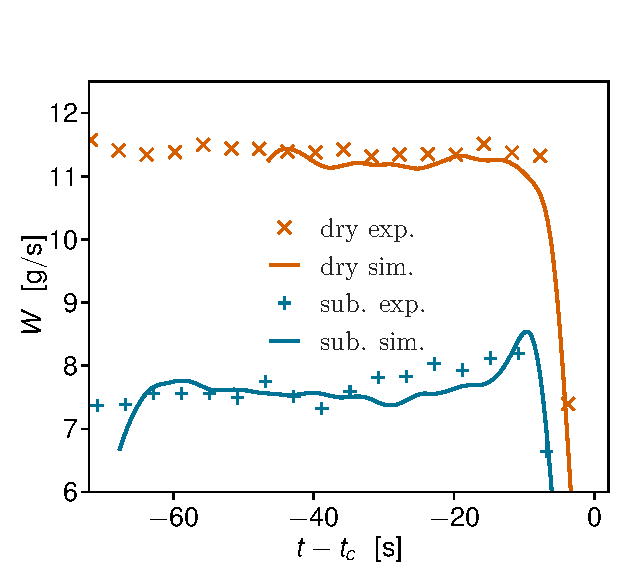
\includegraphics[width=\columnwidth]{fig9-w_vs_t.pdf}\\
 \caption{The derivative of hopper mass over time shows the surge in submerged case for both experiments (blue +) and simulations (solid curve). The surge is not seen in the dry experiments (red x) and simulations (solid red). However, the final moments of the dry experiment might contain a tiny surge that is too fast for the current experimental procedure and analysis.}
 \label{fig:derivated_data}
\end{figure}
\DIFaddend 

\DIFaddbegin {\DIFadd{Flow sensitivity to friction coefficient gives}}
\DIFadd{the possibility to interpret the hopper flow in the context of non-linear effective rheology.
}{\DIFadd{Fig.~\ref{fig:DST} shows a schematic illustration of three systems with (discontinuous) shear thickening \mbox{%DIFAUXCMD
\cite{Peters2016}}\hspace{0pt}%DIFAUXCMD
, a characteristic of frictional granular systems. For the same load, caused by the high particle column, the frictionless case, a Newtonian fluid, has the smallest slope and thus lowest effective viscosity. Friction increases the slope and introduces a sudden increase of viscosity, that can be many orders of magnitude.
When the mass $m(t)$ of the particle column decreases in time, the effective viscosity of the system decreases as well, causing an increase in the flow rate. This is seen as the terminal surge. }}


\DIFaddend \section{Conclusions}

We performed experiments and simulations on dry and submerged hopper 
flows of granular particles of approximately millimeter radius using the 
combination of DEM and CFD. 
In the \DIFaddbegin \DIFadd{dry }\DIFaddend frictionless case, we confirm the previously known numerical result 
\cite{Langston1994}, that the flow rate of the dry granular particles 
decreases as a function of time. 
\DIFdelbegin \DIFdel{Here, we have extended the result of decreasing flow rate to submerged
conditions}\DIFdelend \DIFaddbegin {\DIFadd{In addition, we find the same behavior also for the frictionless submerged
system}\DIFaddend . This scenario \DIFdelbegin \DIFdel{, which occurs in both dry and submerged system could be }\DIFdelend \DIFaddbegin \DIFadd{could be }}
\DIFaddend understood in the context of a Newtonian fluid running out of a hopper.

\DIFdelbegin \DIFdel{The grain-grain friction changes the scenario from a Newtonian behavior into a more complex one: In the dry case the
grain }\DIFdelend \DIFaddbegin {\DIFadd{For dry frictional particles we confirm that the
}\DIFaddend flow rate remains constant until the height of the granular column is less than the width of the hopper \cite{Nedderman1982}.
\DIFdelbegin \DIFdel{This is a well understood behavior , and is }\DIFdelend \DIFaddbegin \DIFadd{Thus, the grain-grain friction changes the scenario from a Newtonian behavior into a more complex one,
}\DIFaddend readily described by the Beverloo equation.\DIFaddbegin }
%DIF > 
\begin{figure}[!t] % figure 10 rheology schematic
 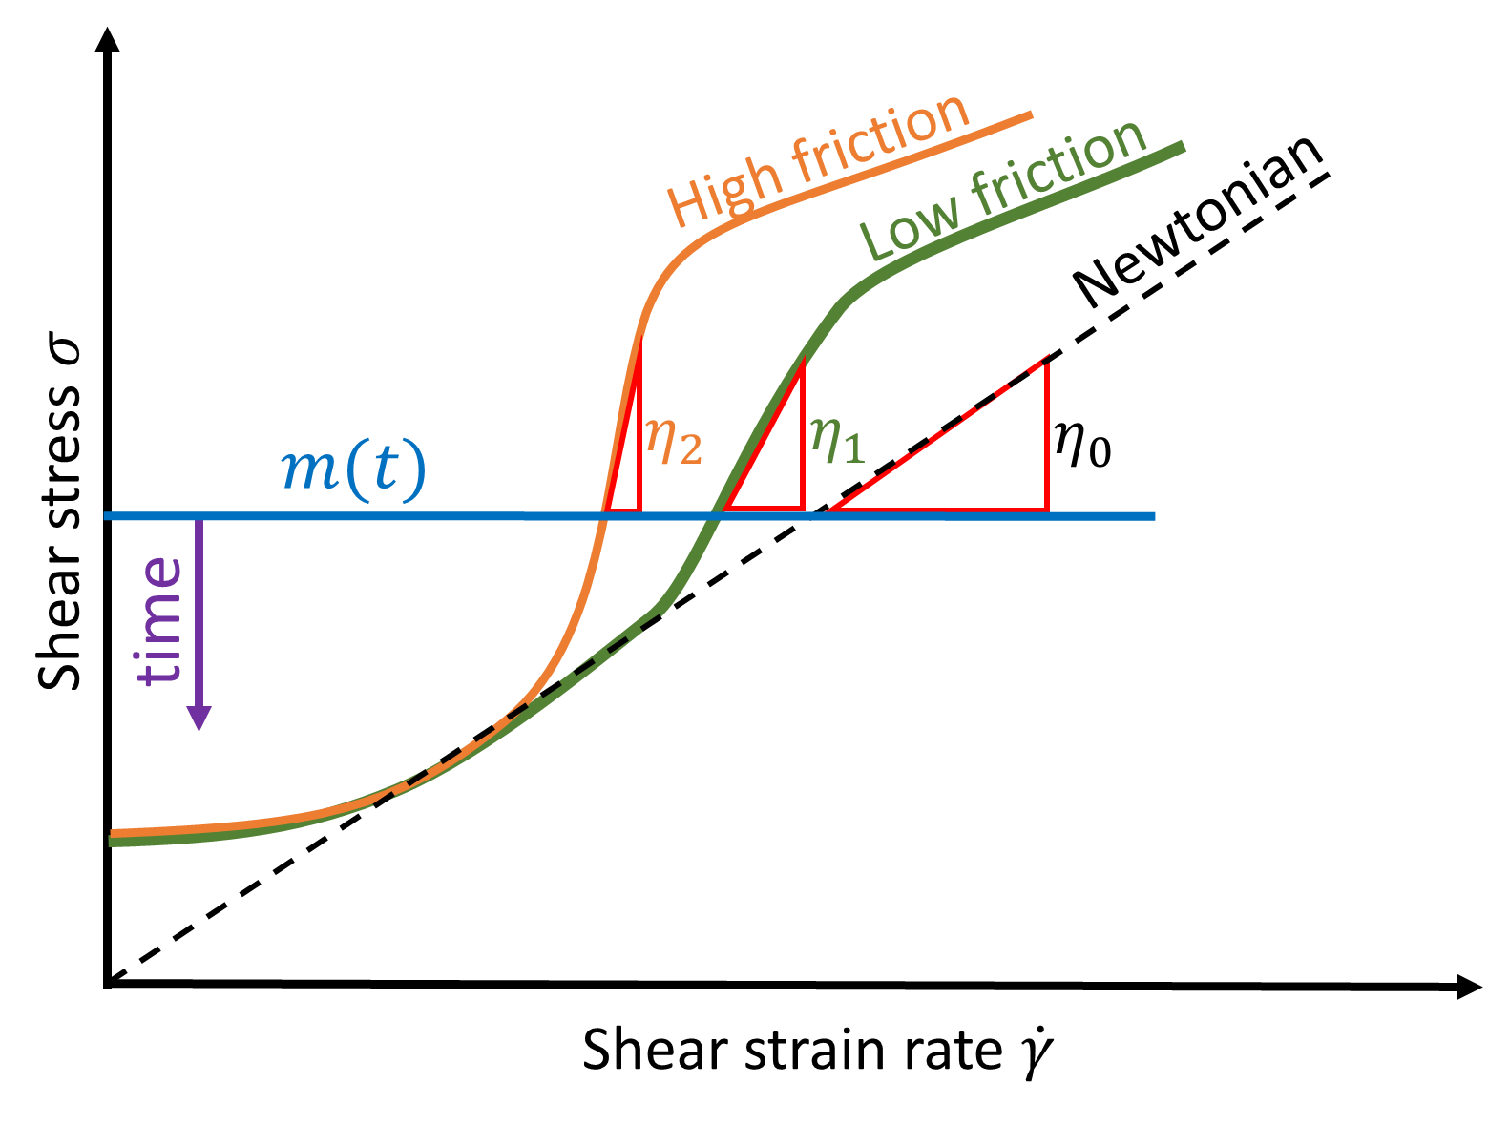
\includegraphics[width=\columnwidth]{fig10-rheology_schematic.pdf}\\
 \caption{A schematic illustration of three materials with discontinuous shear thickening. The increasing contact friction of the particles leads to decreasing flow rate. At continuum, this can be interpreted as increasing effective viscosity $\eta_{i}$ that increases with particle friction for high shear stresses.}\label{fig:DST}
\end{figure}
\DIFaddend 

%DIF < figure rheology schematic
\DIFdelbegin %DIFDELCMD < \begin{figure}[!t] 
%DIFDELCMD <  \includegraphics[width=\columnwidth]{fig9-rheology_schematic.pdf}\\
%DIFDELCMD <  \caption{A schematic illustration of three materials with discontinuous shear thickening. The increasing contact friction of the particles leads to decreasing flow rate. At continuum, this can be interpreted as increasing effective viscosity $\eta_{i}$ that increases with particle friction for high shear stresses.}%DIFDELCMD < \label{fig:DST}%%%
%DIFDELCMD < \end{figure}
%DIFDELCMD < 

%DIFDELCMD < %%%
\DIFdelend In the submerged hopper case, the grain-grain friction \DIFdelbegin \DIFdel{has an even more profound effect. The 
flow accelerates, surging }\DIFdelend \DIFaddbegin \DIFadd{causes the flow to accelerate }\DIFaddend through the whole
hopper emptying process. Furthermore,
right before the hopper runs out of grains there is a clear terminal surge in the flow rate. The
accelerating flow can be understood \DIFdelbegin \DIFdel{in the framework }\DIFdelend \DIFaddbegin \DIFadd{via a simple scenario }\DIFaddend of a feedback loop mediated by the
incompressible, viscous water\DIFdelbegin \DIFdel{. }\DIFdelend \DIFaddbegin \DIFadd{: }\DIFaddend The grains exit the hopper as the gravity pulls them. 
\DIFdelbegin \DIFdel{The grains replace a certain volume of wateroutside the hopper. Due to 
the water incompressibility the same amount of water needs to enter the hopper . This mainly occurs }\DIFdelend \DIFaddbegin \DIFadd{Outside the hopper, the grains replace water, which due to 
the incompressibility enters the hopper mainly }\DIFaddend through the open top \DIFdelbegin \DIFdel{, }\DIFdelend where the flow resistance is the smallest. 
\DIFdelbegin \DIFdel{That }\DIFdelend \DIFaddbegin \DIFadd{This }\DIFaddend creates a flow of water through the granular packing\DIFdelbegin \DIFdel{, which in turnmediated by the viscosity, increases the }\DIFdelend \DIFaddbegin \DIFadd{. It, in turn, due to the viscous drag, pulls
more grains out from the hopper increasing the }\DIFaddend outflow of the
grains. This granular pumping effect is described in \cite{koivistoSubmitted} and is captured by the 
simulation here. 

As we observe, both the dry and submerged cases are sensitive to the grain-grain friction.
This allows us to use the parameter to fit the simulated flow rates against the corresponding 
\DIFaddbegin {\DIFaddend experiments. Subsequently, we observe that the \DIFdelbegin \DIFdel{optimal }\DIFdelend \DIFaddbegin \DIFadd{best fit }\DIFaddend friction parameter is almost\DIFaddbegin }
\DIFaddend the same in both the cases. This was a surprising result, since one would expect the grain-grain
\DIFaddbegin {\DIFaddend friction to be significantly lower \DIFdelbegin \DIFdel{on a wet surface}\DIFdelend \DIFaddbegin \DIFadd{between the grains}\DIFaddend . However, as we do not explicitly account for the grain-grain hydrodynamic interactions, we expect the
friction coefficient to partly compensate for that.\DIFdelbegin \DIFdel{This sensitivity to friction coefficient gives
the possibility to interpret the hopper flow in the context of non-linear effective rheology.
}\DIFdelend \DIFaddbegin }
\DIFaddend 

\DIFdelbegin \DIFdel{Fig.~\ref{fig:DST} shows a schematic illustration of three systems with (discontinuous) shear thickening \mbox{%DIFAUXCMD
\cite{Peters2016}}\hspace{0pt}%DIFAUXCMD
, a characteristic of frictional granular systems. For the same load, caused by the high particle column, the frictionless case, a Newtonian fluid , has the smallest slope and thus lowest effective viscosity. Friction increases the slope and introduces a sudden increase of viscosity, that can be many orders of magnitude. This is observed here as rapid decrease of flow rate as a function of particle-particle friction.
When the mass $m(t)$ of the particle column decreases in time, the effective viscosity of the system decreases as well, causing an increase in the flow rate}\DIFdelend \DIFaddbegin {\DIFadd{In this paper we show that one can successfully capture both qualitatively and quantitatively this counter intuitive behavior arising in a submerged granular hopper flow using coupled discrete element model (DEM) for the particle dynamics and computational fluid dynamics (CFD) for the liquid. While the particle trajectories and interactions are computed explicitly in the DEM-implementation, the fluid flow is modeled on a continuum level by the CFD approach}\DIFaddend . This is \DIFdelbegin \DIFdel{seen as the terminal surge. For a system of high interparticle friction this has a greater impact.}\DIFdelend \DIFaddbegin \DIFadd{fundamentally different from the inertial $\mu(I_v)$-model where the granular media and the interstitial fluid is treated as a single continuum \mbox{%DIFAUXCMD
\cite{Boyer11PRL}}\hspace{0pt}%DIFAUXCMD
.}}
\DIFaddend 

\DIFaddbegin {\DIFaddend Here we have presented the first step to compare simulations \DIFdelbegin \DIFdel{to the experiments }\DIFdelend \DIFaddbegin \DIFadd{and experiments of a submerged hopper flow }\DIFaddend with a good \DIFaddbegin }
\DIFaddend agreement. The one-to-one match with experiments and simulation is currently pushing the 
limits of both methods.
Using smaller than $d=0.2$~cm particles increases the experimental accuracy via lowering the flow rate. 
\DIFdelbegin \DIFdel{However }\DIFdelend \DIFaddbegin {\DIFadd{However, }\DIFaddend using smaller particles \DIFdelbegin \DIFdel{renders the simulation }\DIFdelend \DIFaddbegin \DIFadd{in the simulations renders them }\DIFaddend impractical by making the problem too large for the present computational resources.
Both of these problems, the experimental and numerical \DIFdelbegin \DIFdel{are }\DIFdelend \DIFaddbegin \DIFadd{may be }\DIFaddend solvable in the near future by advanced computational methods \DIFdelbegin \DIFdel{and measurement techniques}\DIFdelend \DIFaddbegin \DIFadd{such as coarse graining of particles in the bulk \mbox{%DIFAUXCMD
\cite{Bierwisch2009MPS, QueteschinerCFD17} }\hspace{0pt}%DIFAUXCMD
and experimental measurement techniques such as identifying and counting individual particles}\DIFaddend . 
Future studies \DIFdelbegin \DIFdel{should }\DIFdelend \DIFaddbegin \DIFadd{could }\DIFaddend involve 
the effect of wall and bottom friction, dilation of grains at the orifice, clogging, self-generated pumping of fluid, terminal and exit velocities of particles\DIFdelbegin \DIFdel{. 
Also, 
we would like to point out that }\DIFdelend \DIFaddbegin \DIFadd{, 
and }\DIFaddend the behavior of \DIFdelbegin \DIFdel{the flow rate at infinitely 
tall packings, the constant component }\DIFdelend $W_{go}$ as \DIFdelbegin \DIFdel{the }\DIFdelend \DIFaddbegin \DIFadd{a }\DIFaddend function of particle size\DIFdelbegin \DIFdel{is also interesting.
There is }\DIFdelend \DIFaddbegin \DIFadd{.
For $W_{go}$ there should be }\DIFaddend a transition from colloidal no-flow behavior to surging flow and back to no-flow 
at clogging, \DIFdelbegin \DIFdel{but this is }\DIFdelend \DIFaddbegin \DIFadd{which unfortunately fell }\DIFaddend outside the scope of this paper\DIFaddbegin \DIFadd{.}}

\section{\DIFadd{Conflicts of interest}}

\DIFadd{There are no conflicts to declare}\DIFaddend .

\section{Acknowledgement}

This work was supported by the Academy of Finland
through the COMP Centre of Excellence and the project
number 278367. The simulations were performed using
the computer resources within the Aalto University
School of Science, Science-IT project. JK acknowledges 
the support from Finnish Cultural Foundation and Wihuri 
foundation through Foundations' Post Doc Pool project. 
DJD acknowledges the support from NFS through grant 
DMR-1305199.


%%%REFERENCES%%%
\bibliography{master} %You need to replace "rsc" on this line with the name of your .bib file
\bibliographystyle{rsc} %the RSC's .bst file

\end{document}
